%%% Для сборки выполнить 2 раза команду: pdflatex <имя файла>

\documentclass[a4paper,12pt]{article}

\usepackage{ucs}
\usepackage[utf8x]{inputenc}
\usepackage[russian]{babel}
%\usepackage{cmlgc}
\usepackage{graphicx}
\graphicspath{ {./images/} }
\usepackage{listings}
\usepackage{xcolor}
\usepackage{hyperref}
\hypersetup{
    colorlinks=true,
    linkcolor=black,
    filecolor=black,      
    urlcolor=cyan,
    pdftitle={НИР},
    pdfpagemode=FullScreen,
    }
%\usepackage{courier}

\makeatletter
\renewcommand\@biblabel[1]{#1.}
\makeatother

\newcommand{\myrule}[1]{\rule{#1}{0.4pt}}
\newcommand{\sign}[2][~]{{\small\myrule{#2}\\[-0.7em]\makebox[#2]{\it #1}}}

% Поля
\usepackage[top=20mm, left=30mm, right=10mm, bottom=20mm, nohead]{geometry}
\usepackage{indentfirst}

% Межстрочный интервал
\renewcommand{\baselinestretch}{1.50}


\begin{document}

%%%%%%%%%%%%%%%%%%%%%%%%%
%%%                   %%%
%%% Титульный лист    %%%

\thispagestyle{empty}
\begin{center}


\renewcommand{\baselinestretch}{1}
{\large
{\sc Петрозаводский государственный университет\\
Институт математики и информационных технологий\\
	Кафедра Информатики и Математического Обеспечения
}
}

\end{center}


\vfill

\begin{center}
{\normalsize Отчет о научно-исследовательской работе} \\

\medskip

%%% Название работы %%%
	{\Large \sc Разработка шаблонов веб-страниц для веб-сервиса коллективных переводов} \\
\end{center}

\medskip

\begin{flushright}
\parbox{11cm}{%
\renewcommand{\baselinestretch}{1.2}
\normalsize
	Выполнила:\\
студентка 2 курса группы 22205
\begin{flushright}
	 С. Э. Зименкова \sign[подпись]{4cm}
\end{flushright}




Научный руководитель:\\
%%% степень, звание ФИО научного руководителя %%%
% Первый руководитель 
Д. Б. Чистяков \\
\begin{flushright}
\sign[подпись]{4cm}
\end{flushright}

Итоговая оценка \\
\begin{flushright}
\sign[оценка]{4cm}
\end{flushright}

% Второй руководитель 
% И. О. Фамилия, ученая степень, ученое звание \\
% \begin{flushright}
% \sign[подпись]{4cm}
% \end{flushright}
}
\end{flushright}

\vfill

\begin{center}
\large
    Петрозаводск --- 2023
\end{center}

%%% Титульный лист    %%%
%%%                   %%%
%%%%%%%%%%%%%%%%%%%%%%%%%


%%%%%%%%%%%%%%%%%%%%%%%%%
%%%                   %%%
%%% Содержание        %%%

\newpage

\tableofcontents

%%% Содержание        %%%
%%%                   %%%
%%%%%%%%%%%%%%%%%%%%%%%%%


%%%%%%%%%%%%%%%%%%%%%%%%%
%%%                   %%%
%%% Введение          %%%

\newpage
\section*{Введение}
\addcontentsline{toc}{section}{Введение}

Перевод больших массивов текста зачастую является трудоемкой задачей, требующей большого количества времени. Задача усложняется, если необходимо перевести художественное произведение, научную работу, текст выступления на конференции или справочные материалы, содержащие большое количество специальной лексики. Процесс перевода становится более эффективным, если он выполняется коллективом профессионалов, выполняющих разные роли: помимо самих переводчиков в работе принимают участие редакторы и руководители проекта, которым нужно разделять обязанности между работниками, согласовывать процесс и утверждать прошедшие редакцию главы. \\

Профессиональный перевод не является единственной возможной формой работы над текстом на иностранном языке. Не все заказчики могут позволить себе оплатить профессиональный перевод значительного по объему текста. Примером подобных текстов могут выступать интерфейс ПО и компьютерных игр, узконаправленная литература, конспекты лекций и конференций, субтитры к видеоматериалам, находящимся в открытом доступе. Такую работу часто выполняют волонтеры, не все из которых обладают достаточными навыками для выполнения профессионального перевода. В проектах, связанных с любительским переводом, помимо синхронизации и распределения частей текста между участниками, необходимо проверять качество работы и выбирать наилучшие варианты перевода, так как волонтеры и любители не несут достаточной ответственности за свою работу и не могут гарантировать его верность. \\

Решением проблемы распределения, синхронизации и утверждения перевода для команд переводчиков любой степени профессионализма является удобный инструмент, позволяющий пользователям совместно работать над переводом.\\
Предложенный инструмент будет реализован в форме веб-сервиса, позволяющего пользователям:
\begin{itemize}
	\item Создавать новые проекты и принимать участие в существующих проектах:
	\begin{description}
		\item[-] Пользователь может создать проект, присвоить ему свойства, добавить описание, сделать проект открытым или закрытым для других пользователей, приглашать других пользователей стать участниками проекта, разрешать другим пользователям становиться участниками проекта.
		\item[-] Пользователь может искать открытые проекты, оставлять заявку на участие в них и принимать участие после одобрения заявки руководителем проекта; получать доступ по ссылке к закрытым проектам и принимать в них участие после одобрения заявки руководителем проекта; принимать участие в проектах, в которые был приглашен.
	\end{description}
	\item Разбивать исходный текст на отдельные главы, а главы на отдельные фрагменты:
	\begin{description}
		\item[-] Пользователь может использовать автоматическое разбиение на фрагменты по переносам строки или вручную задавать разбиение текста.
	\end{description}
	\item Распределять роли между участниками проекта:
	\begin{description}
		\item[-] В проекте существуют роли, которые присваиваются участникам. В зависимости от роли участник может выполнять различные функции и действия. Например, роль редактора позволяет участнику утверждать верный вариант перевода и вносить правки в итоговый результат, роль руководителя проекта позволяет участнику назначать другие роли и выполнять все доступные действия.
	\end{description}
	\item Распределять работу над фрагментами между участниками проекта:
	\begin{description}
		\item[-] В проекте есть возможность создавать связь между фрагментом текста и участником, выполняющим перевод этого фрагмента. Эта функция позволяет по необходимости исключить выполнение перевода двумя разными участниками, что повышает эффективность за счет сокращения потраченного на выполнение лишней работы времени.
	\end{description}
	\item Предлагать варианты перевода каждого фрагмента:
	\begin{description}
		\item[-] Участник проекта может добавить вариант перевода этого фрагмента. Все предложенные варианты перевода доступны для прочтения другим участникам проекта.
	\end{description}
	\item Рецензировать и редактировать перевод:
	\begin{description}
		\item[-] Путем голосования наиболее верным вариантом считается тот, который получил наибольшее количество голосов от участников. Между вариантами с одинаковым количеством голосов выбирается тот, который был составлен позже.
		\item[-] Участники с более высокими ролями (редактор, руководитель проекта) могут выбрать лучший на свой взгляд вариант перевода вне зависимости от итогов голосования. Решение участника с более высокой ролью превалирует над решением участника с менее высокой ролью.
	\end{description}
	\item Сохранять итоговый результат:
	\begin{description}
		\item[-] Итоговый результат может быть получен в различном виде. Кроме формата полученного файла можно также выбрать, какой перевод будет вставлен в итоговый файл. Эти параметры будут настраевыми при экспорте перевода.
	\end{description}
\end{itemize}

Разработка веб-сервиса, подходящего для работы профессионалов, будет разделена на три этапа:
\begin{itemize}
	\item разработка структуры (веб-API, база данных) и веб-страниц;
	\item установка связи между back-end и front-end составляющими проекта, разработка инструмента-редактора;
	\item доработка и улучшение сервиса, расширение функционала.\\
\end{itemize}

Цель данной работы — разработка шаблонов веб-страниц для описанного сервиса. Это необходимо, чтобы ускорить и упростить будущую разработку. Программный код будет работать с сервером, получая и передавая ему информацию, на основе которой будут строиться веб-страницы. Чтобы заранее понимать, как объекты будут расположены на странице, оценить их эстетическую привлекательность и не тратить время на веб-дизайн в процессе написания скриптов на языке программирования, нужно разработать статические шаблоны будущих страниц, которые можно будет копировать и вставлять в программный код с незначительными изменениями.

Для осуществления поставленной цели необходимо выполнить следующие задачи:
\begin{itemize}
	\item исследовать существующие веб-сервисы и сделать выводы о необходимом функционале и подходящем дизайне интерфейса;
	\item изучить существующие инструменты и технологии для разработки веб-страниц, выбрать наиболее подходящие для реализации проекта;
	\item разработать удобные и визуально привлекательные шаблоны веб-страниц.
\end{itemize}

%%% Введение          %%%
%%%                   %%%
%%%%%%%%%%%%%%%%%%%%%%%%%



%%%%%%%%%%%%%%%%%%%%%%%%%
%%%                   %%%
%%% Глава 1           %%%

\newpage
\section{Анализ предметной области}
\subsection{Необходимые данные для разработки веб-страниц}

Веб-дизайн — вид графического дизайна, направленный на разработку и оформление объектов информационной среды интернета, призванный обеспечить им высокие потребительские свойства и эстетические качества. Подобная трактовка отделяет веб-дизайн от веб-программирования, подчеркивает специфику предметной деятельности веб-дизайнера, позиционирует веб-дизайн как вид графического дизайна \cite{book:web}. Для создания визуально привлекательного и удобного интерфейса необходимо иметь соответствующие навыки или образование, но в случае их отсутствия все равно возможно создать удобный пользовательский интерфейс. Для этого существуют специальные инструменты (фреймворки, библиотеки), предоставляющие разработчику набор готовых элементов, визуально сочетающихся между собой. UX/UI-дизайн — работа одного или даже двух разных специалистов, но не имея опыта в сфере UX/UI-дизайна, можно опираться на широко распространенные среди других сервисов шаблоны внешнего вида и конструкции интерфейса.\\
Фреймворк (англ. framework — «каркас, структура») — готовый набор инструментов, который помогает разработчику быстро создать продукт: сайт, приложение, интернет-магазин, CMS-систему. \cite{website:yandex1}\\
UX (англ. user experience — «пользовательский опыт») — то, каким образом пользователь взаимодействует с интерфейсом и насколько сайт или приложение для него удобны. В UX входит навигация по сайту, функционал меню и результат взаимодействия со страницами. UI (англ. user interface — «пользовательский интерфейс») — оформление сайта: сочетания цветов, шрифты, иконки и кнопки. \cite{website:skillbox1}\\

Таким образом, чтобы разработать удобный и визуально привлекательный веб-сайт, нужно изучить существующие веб-сайты и узнать, как на них выглядят и располагаются элементы интерфейса, а также изучить доступные фреймворки и библиотеки, которые упростят разработку интерфейса.

\subsection{Описание существующих инструментов для коллективных переводов}

Существует несколько сервисов для работы с коллективным переводом. В этом разделе будут описаны примеры существующих веб-сервисов, которые были изучены, чтобы узнать, какие элементы интерфейса и функционал уже используются для работы с коллективными переводами, и каких функций не хватает в этих сервисах.\\

\subsubsection{Crowdin.com}
Crowdin.com — облачное решение, созданное для локализации программных продуктов и документации для них.  \cite{website:crowdin}\\
Из всех рассмотренных примеров веб-сервис Crowdin.com предоставляет наиболее широкий функционал и больше всего удобных инструментов для пользователей. Данный веб-сервис обладает следующими преимуществами:
\begin{itemize}
	\item[+] Поддержка большого разнообразия форматов входных файлов и расширений;
	\item[+] Встроенный переводчик, предлагающий несколько вариантов переводов для пользователя;
	\item[+] Готовые решения для разработчиков, маркетологов, дизайнеров и переводчиков;
	\item[+] Удобные инструменты для локализации программного обеспечения, веб-сайтов, мобильных приложений, пользовательского интерфейса;
	\item[+] Инструменты для отслеживания прогресса работы над переводом.
\end{itemize}

У этого веб-сервиса также есть недостатки:
\begin{itemize}
	\item[-] Данный веб-сервис предназначен для локализации программного обеспечения, веб-сайтов и документации, но он не так удобен для переводов литературных произведений;
	\item[-] Веб-сервис обладает широким функционалом, но не имеет достаточно интуитивного дизайна. Пользователю необходимо некоторое время потратить на регистрацию, прежде чем он сможет переключить язык сайта с английского на русский или любой другой. Слишком большое количество инструментов, которыми пользователь, вероятно, не будет пользоваться;
	\item[-] Главный недостаток — Crowdin.com является коммерческим проектом. Это означает, что он не подходит для переводчиков-любителей и энтузиастов, желающих помочь с переводом какого-либо произведения, и не имеющих возможности оплатить работу с инструментом.
\end{itemize}

\subsubsection{Notabenoid.org}

Notabenoid.org — веб-сервис, нацеленный на коллективные любительские переводы программ, книг и субтитров к фильмам. \cite{website:nota}\\
Проект Notabenoid стал закрытым в 2014 году и с тех пор не поддерживается разработчиком.\\

Преимущества этого веб-сервиса:
\begin{itemize}
	\item[+] Поддержка текстовых форматов входных файлов и файлов субтитров;
	\item[+] Удобный интуитивный дизайн;
	\item[+] Возможность публиковать проекты и привлекать больше людей для работы над ними;
	\item[+] Публичные переводы разделены на категории и жанры;
	\item[+] Сервис бесплатный для всех пользователей.
\end{itemize}

Основные недостатки этого веб-сервиса:
\begin{itemize}
	\item[-] Из-за того, что веб-сервис значительное количество времени не поддерживается разработчиком, он сильно устарел. Функционал инструмента не расширяется, очень малое количество людей пользуется этим веб-сайтом, при возникновении ошибки нет возможности обратиться к разработчику;
	\item[-] Малое разнообразие поддерживаемых файлов;
	\item[-] Есть недостатки в дизайне самого инструмента для работы с фрагментами переводов;
	\item[-] Сервис закрыт для большинства людей в интернете, пользоваться им можно только после получения приглашения от одного из зарегистрированных участников.
\end{itemize}

\subsubsection{Transifex.com}

Transifex.com — веб-сервис для локализации программного обеспечения, документации, веб-сайтов и субтитров. \cite{website:transifex}\\
Он очень похож на Crowdin.com, поэтому обладает теми же преимуществами: современный дизайн, множество удобных инструментов для работы, инструкции и готовые решения. Однако сервис узконаправлен и предназначен для перевода ПО и веб-сайтов, поэтому не подходит для перевода литературы, а также является коммерческим проектом, не имеющим бесплатной версии, из-за чего не подходит для любительских переводов и небольших проектов.

\subsubsection{Translatewiki.net}

Translatewiki.net — сообщество локализации проектов с открытым исходным кодом. Этот веб-сервис имеет очень специфичное предназначение — локализация вики-страниц, т. к. работает на основе расширения "Перевод"\ для Медиавики. \cite{website:wiki}\\
Сервис бесплатный, обладает удобным и простым интерфейсом, широко используем для проектов с открытым исходным кодом, но не подходит для перевода и локализации чего-либо, кроме вики-проектов, поэтому не подходит для решения поставленной проблемы.

\subsubsection{Weblate}
Weblate — облачное решение для локализации проектов по разработке ПО. \cite{website:weblate}

Этот инструмент обладает следующими преимуществами:
\begin{itemize}
	\item[+] Поддержка большого разнообразия форматов файлов;
	\item[+] Удобный современный дизайн;
	\item[+] Полная интеграция перевода и система контроля версий;
	\item[+] Поддержка площадок для совместной работы (например, GitHub);
	\item[+] Удобные инструменты для отчетности, отслеживания прогресса, продвижения проекта.
\end{itemize}

Однако, у этого сервиса есть недостатки:
\begin{itemize}
	\item[-] Предназначен для локализации программного кода и не подходит для переводов любых иных проектов;
	\item[-] Коммерческий проект — необходимо оплачивать Weblate как услугу, если у пользователя нет собственного хостинга;
	\item[-] Не предназначен для любительских переводов.
\end{itemize}

\subsection{Общие черты в дизайне и функционале рассмотренных сервисов}
У всех рассмотренных сервисов есть общие черты в дизайне и функциональных возможностях:
\begin{itemize}
	\item Минималистичный дизайн пользовательского интерфейса;
	\item Разделение исходного текста на фрагменты для перевода;
	\item Поддержка разных форматов входных данных;
\end{itemize}
Некоторые сервисы объединяли такие функции, как голосование за лучший вариант перевода, анализ прогресса и активности.\\
Большинство этих проектов не поддерживают перевод художественных произведений и импорт некоторых текстовых форматов. Часть из них платные и недоступны для переводчиков-любителей. Большинство из них предназначены для узконаправленной локализации и недостаточно универсальны.\\

\subsection{Вывод главы}
После рассмотрения дизайна и функционала этих приложений, можно сделать следующие выводы касательно функций и внешнего вида будущего веб-сервиса:
\begin{itemize}
	\item Дизайн сервиса должен быть минималистичным, интуитивным и простым;
	\item Сервис должен предоставлять возможность импортировать разные форматы файлов;
	\item Сервис должен предоставлять возможность переводить тексты для разных проектов и направлений;
	\item Пользователю должна быть предоставлена возможность делать свой проект открытым для сообщества, чтобы увеличить количество переводчиков-энтузиастов в проекте и продвигать его в сообществе, или закрытым, если команда переводит коммерческий проект.
\end{itemize}

Дополнительные функции, например, инструменты для отчетности и анализа активности, можно реализовать позже, так как они необходимы только для коммерческих проектов и на общий функционал сервиса не влияют, являясь потенциальным расширением возможностей.


%%% Глава 1           %%%
%%%                   %%%
%%%%%%%%%%%%%%%%%%%%%%%%%



%%%%%%%%%%%%%%%%%%%%%%%%%
%%%                   %%%
%%% Глава 2           %%%

\newpage
\section{Описание инструментов и технологий}
\subsection{Выбор инструментов для создания шаблонов веб-страниц}
HTML (HyperText Markup Language) — язык разметки, используемый для структурирования и отображения веб-страницы и ее контента. Например, контент может быть структурирован внутри множества параграфов, маркированных списков или с использованием изображений и таблиц данных. HTML не является языком программирования, и используется для того, чтобы сообщить браузеру, как необходимо отображать открытую веб-страницу. HTML-разметка позволяет создавать сколько угодно простые или сложные дизайны пользовательских интерфейсов для любых веб-сайтов. \cite{website:html}\\

CSS (Cascading Style Sheets) — язык таблицы стилей, используемый для применения стилей к элементам в документах HTML. CSS позволяет применять стили к элементам выборочно, используя классы, теги, идентификаторы и так далее. \cite{website:css}\\

Для создания веб-страниц используется HTML-разметка и создание стилей с помощью CSS, но существует множество инструментов для того, чтобы упростить и улучшить процесс разработки веб-страниц. Далее будут приведены примеры некоторых из них. \cite{website:hexlet}
\subsubsection{Bootstrap}
Bootstrap — один из самых популярных инструментов для написания веб-сайтов.\\
Преимущества:
\begin{itemize}
	\item[+] адаптивная сетка: значительно упрощен процесс разделения экрана на части за счет системы из 12 столбцов;
	\item[+] оптимизация для разработки мобильных приложений: принцип mobile-first;
	\item[+] большой набор готовых компонентов, которые автоматически адаптируются под размер экрана;
	\item[+] современный плоский дизайн элементов;
	\item[+] возможность использовать JavaScript в разработке;
	\item[+] обширная качественная документация.
\end{itemize}

Недостатки:
\begin{itemize}
	\item[-] неинтуитивный синтаксис;
	\item[-] большой вес CSS-файлов, что может замедлить первую загрузку страницы.\\
\end{itemize}

Вывод: Bootstrap очень удобен для использования начинающими разработчиками, т. к. имеет большую библиотеку готовых современных дизайнов компонент, качественную документацию и автоматически адаптирует контент на странице под размер экрана пользователя. У этого инструмента есть недостаток — большой вес CSS-файлов, но это влияет только на скорость первой загрузки страницы, а также Bootstrap позволяет настроить, какие части набора будут использоваться.\\

\subsubsection{Tailwind}
Tailwind — CSS-фреймворк, предлагающий пользователю большой каталог классов и инструментов для стилизации сайтов и приложений.\\
Преимущества:
\begin{itemize}
	\item[+] есть возможность создавать собственные свойства и далее использовать их в разработке;
	\item[+] легко настраивается;
	\item[+] интеграция PurgeCSS, позволяющая убрать из CSS-файлов неиспользуемые классы;
	\item[+] множество служебных шаблонов.
\end{itemize}

Недостатки:
\begin{itemize}
	\item[-] слишком большой выбор классов, которые можно использовать в разработке, но скорее всего не будут использованы.\\
\end{itemize}

Вывод: Tailwind предоставляет очень большой набор готовых классов и свойств и позволяет оптимизировать CSS-файлы, однако не очень подходит для веб-разработчиков без достаточно большого опыта, так как имеет действительно много всевозможных классов, которые не нужны начинающему разработчику и могут мешать в процессе работы.

\subsubsection{Material-UI}
Material-UI — библиотека с открытым кодом, которая включает в себя компоненты React, реализующие Material Design от Google.\\
Преимущества:
\begin{itemize}
	\item[+] подробная документация;
	\item[+] регулярные обновления;
	\item[+] единство дизайна компонентов.
\end{itemize}

Недостатки:
\begin{itemize}
	\item[-] мутабельность: библиотека хорошо работает в маленьких проектах, но при росте проекта компоненты начинают мутировать, и это крайне тяжело быстро решить;
	\item[-] проблемы с производительностью: в крупных проектах со сложными алгоритмами и большим количеством компонентов библиотека работает медленно.\\
\end{itemize}

Вывод: Material-UI обладает очень эстетичными компонентами, но не подходит для разработки больших проектов, так как компоненты могут перестать работать должным образом, а сама библиотека становится медленнее при высокой нагрузке.\\

\subsubsection{Foundation}
Foundation — адаптивный интерфейсный фреймворк, разработанный для работы в сочетании с фреймворком Rails для языка Ruby.\\
Преимущества:
\begin{itemize}
	\item[+] большое количество инструментов для веб-разработки;
	\item[+] высокая гибкость и настраиваемость;
	\item[+] множество готовых решений (таблицы, проверка форм, адаптивные элементы).
\end{itemize}

Недостатки:
\begin{itemize}
	\item[-] не поддерживается никакой компанией, только волонтерами;
	\item[-] очень высокая сложность фреймворка: слои, компоненты, большое количество доступных настроек требуют длительного изучения и не подходят для начинающих разработчиков.\\
\end{itemize}

Вывод: Foundation — очень качественный фреймворк, позволяющий полностью настраивать интерфейс, однако нужно очень много времени и практики, чтобы научиться качественно с ним работать, а также он создан для легкой работы с Rails, в то время как для разработки серверной части этого проекта был выбран Node.js.\\

\subsubsection{UIkit}
UIkit — небольшой фреймворк, который специализируется на минимализме в дизайне.\\
Преимущества:
\begin{itemize}
	\item[+] сверхчистые, элегантные и не лишенные пробелов дизайны;
	\item[+] комплект готовых компонентов для различных частей сайтов;
	\item[+] хорошо подходит для очень простых задач, которые нужно быстро решить.
\end{itemize}

Недостатки:
\begin{itemize}
	\item[-] автономная система, поэтому ее нельзя расширять или изменять;
	\item[-] работает со своим JavaScript: использование виртуальной структуры, например, React, невозможно.\\
\end{itemize}

Вывод: UIkit — хороший небольшой фреймворк, который отлично подходит для быстрого решения небольших задач. Тем не менее, он плохо подходит для крупных проектов, т. к. не позволяет работать с распространенными структурами или изменять/расширять сам фреймворк.\\

\subsection{Вывод}
Исходя из преимуществ и недостатков рассмотренных инструментов, библиотек и фреймворков, было принято решение использовать Bootstrap, так как этот набор инструментов широко распространен, подходит для начинающих веб-разработчиков, содержит достаточно готовых компонентов, имеет подробную качественную документацию, а также полностью сочетается с JavaScript.\\


%%% Глава 2           %%%
%%%                   %%%
%%%%%%%%%%%%%%%%%%%%%%%%%



%%%%%%%%%%%%%%%%%%%%%%%%%
%%%                   %%%
%%% Глава 3           %%%

\newpage
\section{Разработка шаблонов веб-страниц}

Для разработки шаблонов веб-страниц использовались HTML5 и Bootstrap v5.3. Основное предназначение созданных веб-страниц — создание дизайна будущего веб-сервиса и готовых HTML-элементов, которые позже можно будет использовать для создания страниц с помощью JavaScript, используя информацию, предоставляемую серверной составляющей сервиса. Готовые элементы можно будет вставить в код без необходимости продумывать, как они будут выглядеть на странице.

Листинги HTML-разметки всех страниц доступны по ссылке:\\
\href{https://github.com/ipaingo/DesmanTranslate}{https://github.com/ipaingo/DesmanTranslate}\\


\subsection{Главная страница}

\begin{figure}[h]
\centering
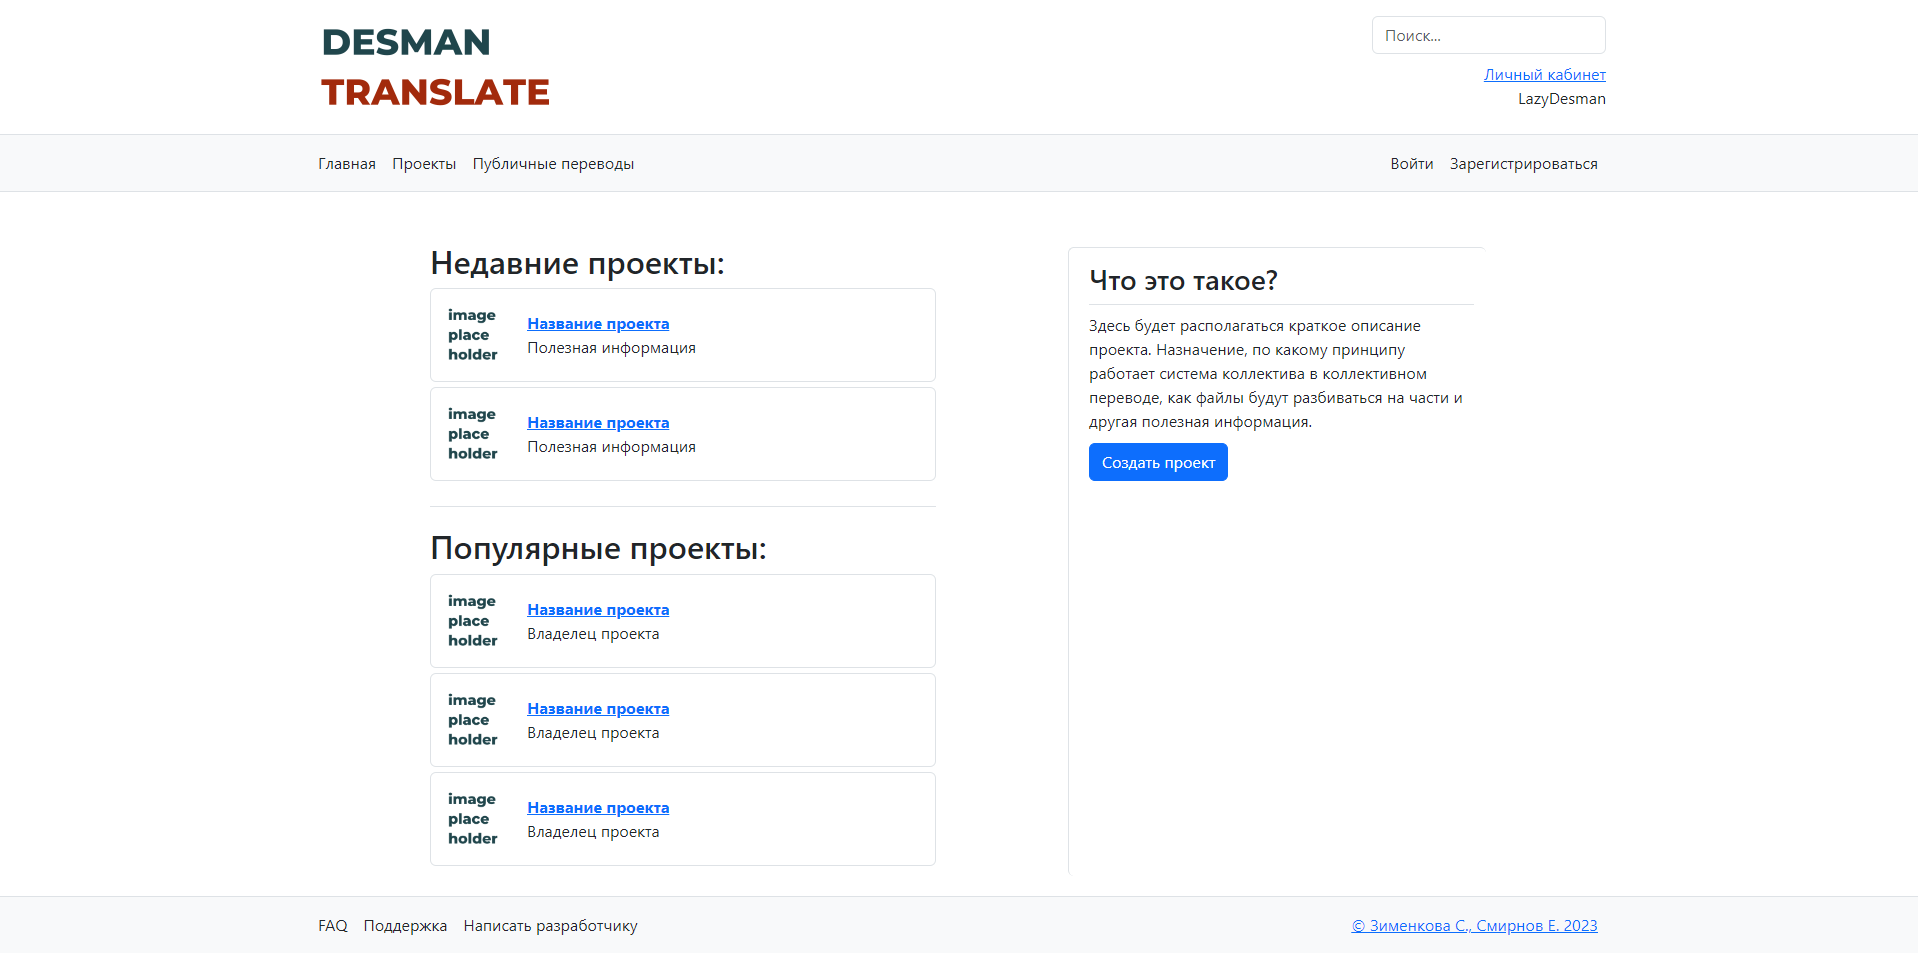
\includegraphics[width=400px]{index.png}
\caption{Главная страница веб-сервиса.}
\label{fig:index}
\end{figure}

В шапке главной странице веб-сайта будут отображаться логотип, навигация по сайту (в качестве примера указаны главная страница, страница проектов пользователя и страница с публичными проектами), а также кнопки дял регистрации и входа, если пользователь не вошел в аккаунт, или же ссылка на личный кабинет пользователя, если пользователь вошел в аккаунт. Шапка страницы и футер внизу страницы (он наполнен примерами ссылок, которые могут быть в футере) повторяются для всех страниц. В основной части страницы расположены ссылки на недавние проекты пользователя, если такие есть, и несколько публичных проектов.\\
На примере главной страницы подробно рассмотрим устройство шаблонов. На рис. \ref{fig:index} показано, как будет выглядеть дизайн главной страницы. На рис. \ref{fig:smallindex} показано, как меняется внешний вид страницы при изменении ширины окна. Bootstrap позволяет легко адаптировать элементы страницы в зависимости от размера экрана. Все стили элементов достигаются путем подключения инструментов Bootstrap в качестве классов для HTML-тегов.

\begin{figure}[h]
\centering
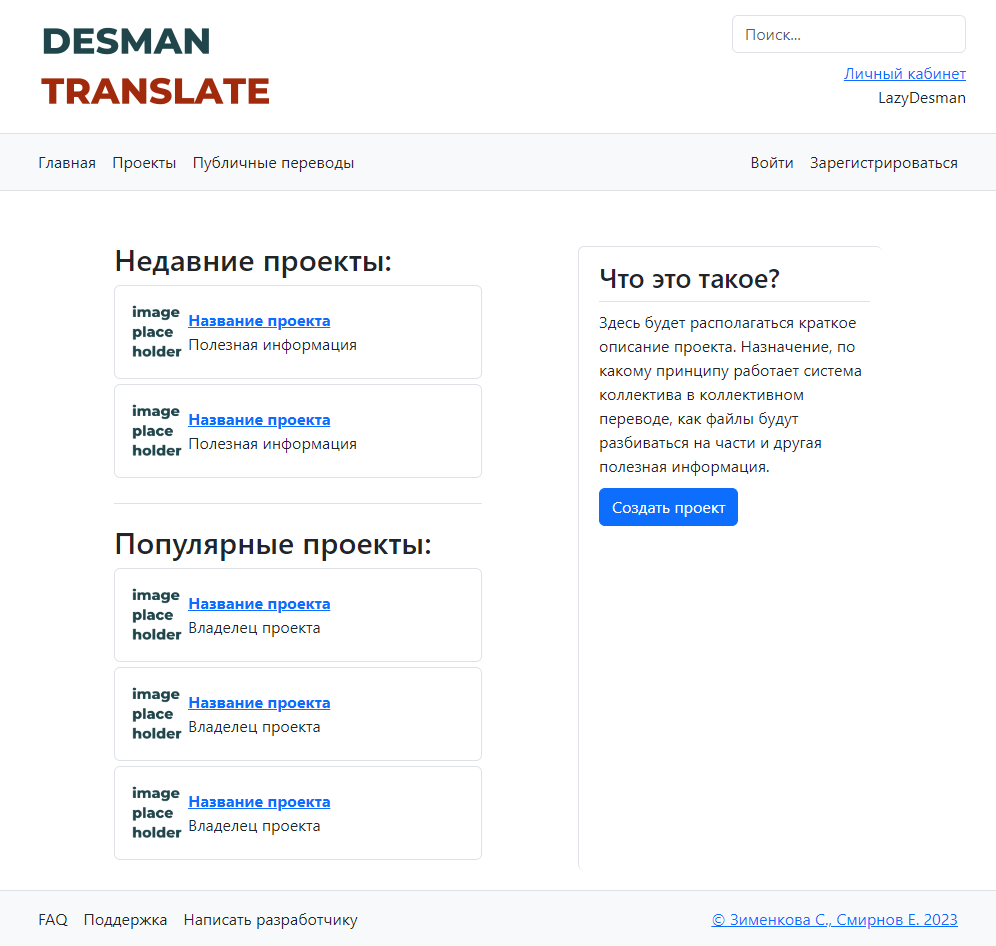
\includegraphics[width=300px]{smallindex.png}
\caption{Главная страница веб-сервиса в окне другого размера.}
\label{fig:smallindex}
\end{figure}

Далее все описываемые рисунки прикреплены в разделе Приложение.\\

\subsection{Страница проектов пользователя}
На странице проектов есть две вкладки. В первой вкладке отображаются проекты, в которых участвует пользователь, кнопка, перенаправляющая пользователя на страницу создания нового проекта, статистика по проектам, в которых участвует пользователь. Во второй вкладке отображаются приглашения, которые пользователь получил от других пользователей, с возможностью принять приглашение и стать участником проета, или же отклонить его. Вкладки страницы с проектами показаны на рис. \ref{fig:projects1} и рис. \ref{fig:projects2}.


\subsection{Страница публичных проектов}
Страница публичных проектов разделена на четыре вкладки: "Популярное", "Фильмы", "Тексты", "Программы". В каждой вкладке будут расположены несколько страниц популярных переводов по разделам, а также блок с фильтром, с помощью которого можно регулировать, какие проекты будут отображаться на странице. На рис. \ref{fig:public1} и рис. \ref{fig:public2} показаны вкладки "Популярное"\ и "Фильмы". Остальные две вкладки выглядят так же.


\subsection{Регистрация и вход}
На рис. \ref{fig:login} и рис. \ref{fig:signup} показаны страницы, на которые пользователь переходит при нажатии на кнопки "Войти"\ и "Зарегистрироваться".


\subsection{Личный кабинет пользователя}
В личном кабинете пользователя, как видно на рис. \ref{fig:user}, на странице личного кабинета есть две вкладки: "О вас"\ и "Настройки". Вкладка "О вас"\ видна всем пользователям, если аккаунт публичный, вкладка "Настройки"\ видна только владельцу личного кабинета.
В первой вкладке расположена основная информация о пользователе, его изображение профиля, проекты, в которых он участвует. Для удобства над списком проектов также помещена кнопка, перенаправляющая пользователя на страницу создания проекта.

Во вкладке "Настройки"\ (рис. \ref{fig:usersettings}) пользователь может изменить основную информацию о себе, сделать свой аккаунт закрытым или открытым. По мере расширения функционала веб-сервиса этих настроек может стать больше.


\newpage
\subsection{Страница проекта}
На рис. \ref{fig:projectpage} показана главная страница проекта. На ней расположена основная информация, оглавление, кнопка, по которой можно перейти к загрузке новой главы. При нажатии на название главы открывается текстовый редактор. На рис. \ref{fig:members} показана страница участников. Только модераторы могут менять роли участников и исключать их. Роль владельца изменить нельзя; владелец проекта меняется в настройках проекта (рис. \ref{fig:settings}), доступных модераторам. Модераторы - владелец и редакторы проекта, имеющие больше возможностей, чем обычные участники проекта (переводчики).


\subsection{Создание нового проекта}
На рис. \ref{fig:newproject} показана форма создания нового проекта. Пользователь переходит на эту страницу, нажав на кнопку "Создать проект"\ на главной странице, на странице проектов или в своем личном кабинете.


\subsection{Добавление глав в существующий проект}
На рис. \ref{fig:addchapter} показана страница, на которую пользователь переходит, нажав на кнопку "Добавить главу"\ в оглавлении на странице проекта. В этой форме пользователь должен ввести название главы, статус главы, и прикрепить файл, из которого будет загружаться текст. Список принимаемых формой файлов можно настроить с помощью HTML-разметки.


%%% Глава 3           %%%
%%%                   %%%
%%%%%%%%%%%%%%%%%%%%%%%%%



%%%%%%%%%%%%%%%%%%%%%%%%%
%%%                   %%%
%%% Заключение        %%%

\newpage
\section*{Заключение}
\addcontentsline{toc}{section}{Заключение}
В результате проделанной работы были изучены существующие сервисы для осуществления коллективных переводов, исследованы их преимущества и недостатки, на их основе были сделаны выводы о том, какие функции необходимы веб-сервису, каких недостатков нужно избежать. Были изучены доступные инструменты и технологии для создания веб-страниц, выбраны оптимальные для данного проекта инструменты. В результате работы были созданы HTML-файлы с шаблонами веб-страниц, которые позволяют проработать внешний вид будущего сервиса, а также упрощают последующую разработку, т. к. все необходимые для генерации страниц элементы были написаны.\\

%%% Заключение        %%%
%%%                   %%%
%%%%%%%%%%%%%%%%%%%%%%%%%



%%%%%%%%%%%%%%%%%%%%%%%%%
%%%                   %%%
%%% Литература        %%%

\newpage
\addcontentsline{toc}{section}{Список литературы}
\bibliographystyle{plain}
\bibliography{refs}

%%%  Литература       %%%
%%%                   %%%
%%%%%%%%%%%%%%%%%%%%%%%%%



%%%%%%%%%%%%%%%%%%%%%%%%%
%%%                   %%%
%%% Приложение        %%%

\newpage
\section*{Приложение}
\addcontentsline{toc}{section}{Приложение}

\begin{figure}[h]
\centering
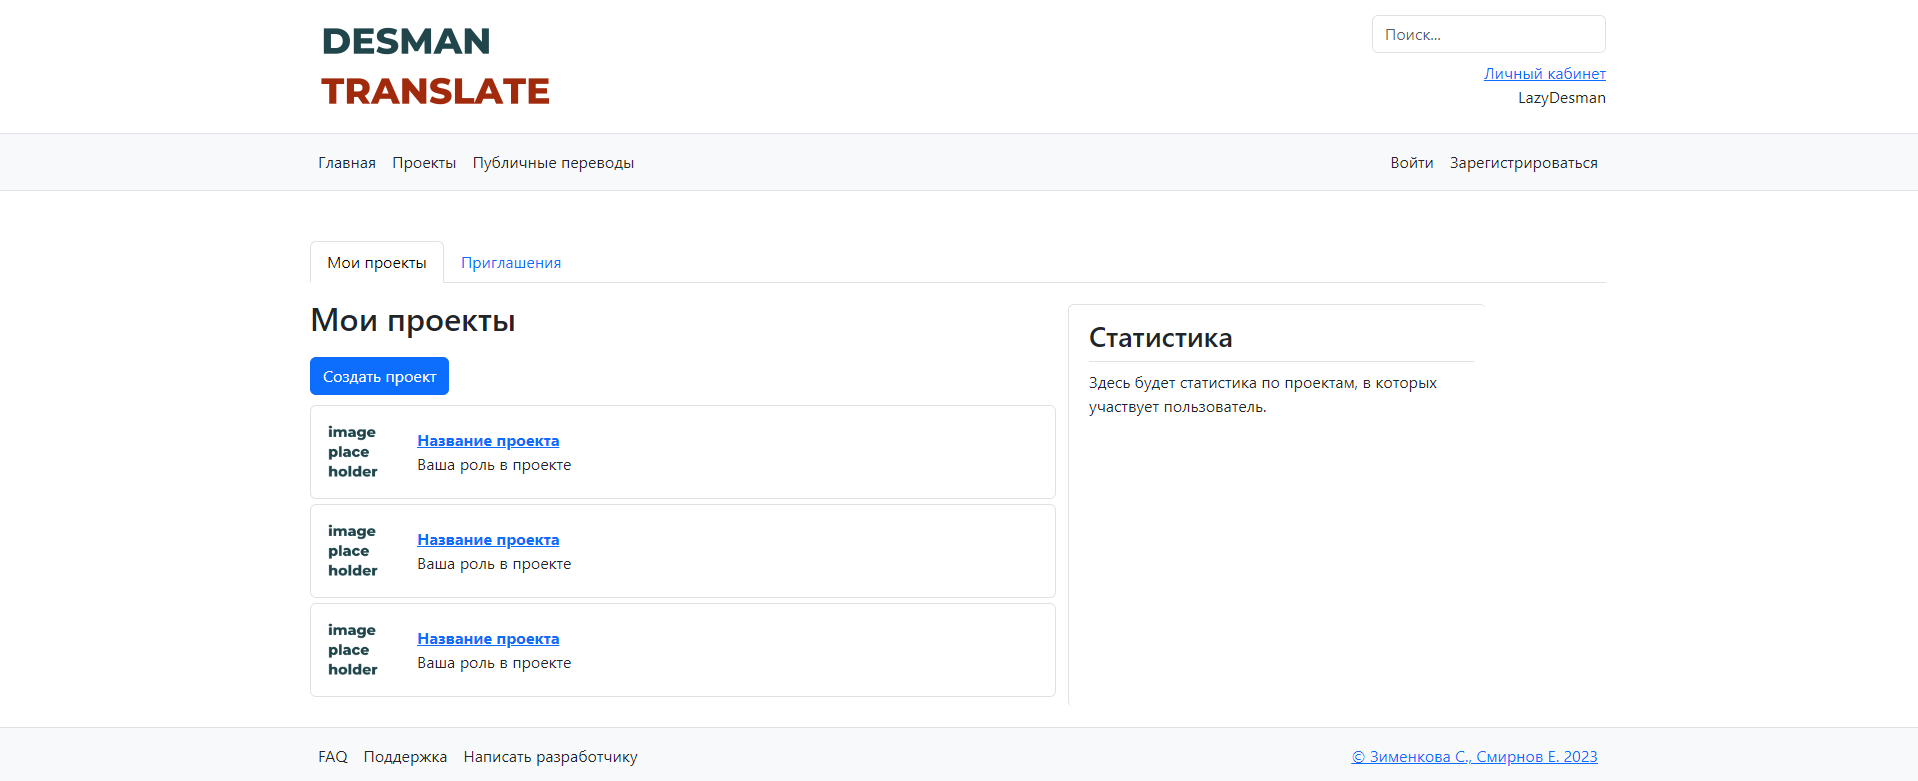
\includegraphics[width=400px]{projects1.png}
\caption{Проекты пользователя.}
\label{fig:projects1}
\end{figure}

\begin{figure}[h]
\centering
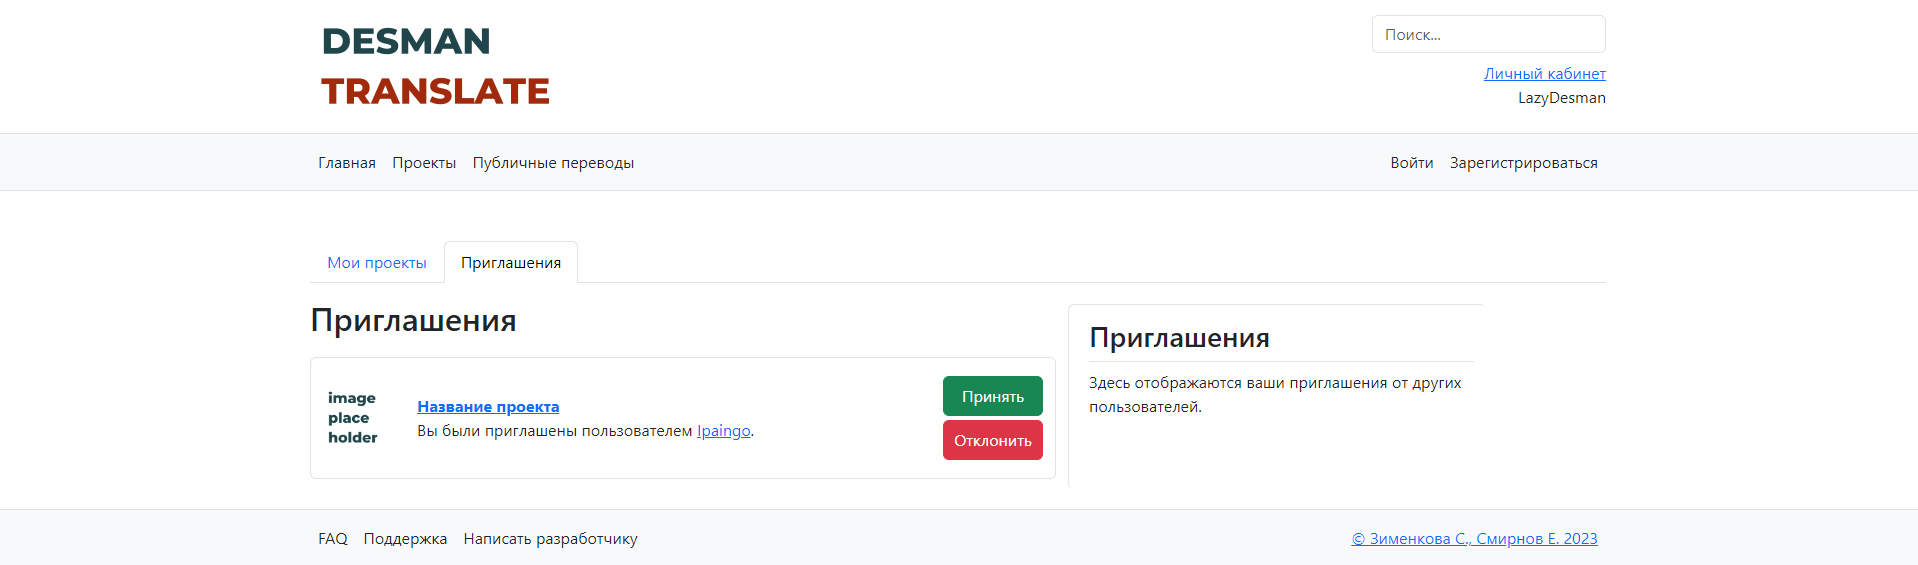
\includegraphics[width=400px]{projects2.png}
\caption{Приглашения пользователя.}
\label{fig:projects2}
\end{figure}

\begin{figure}[h]
\centering
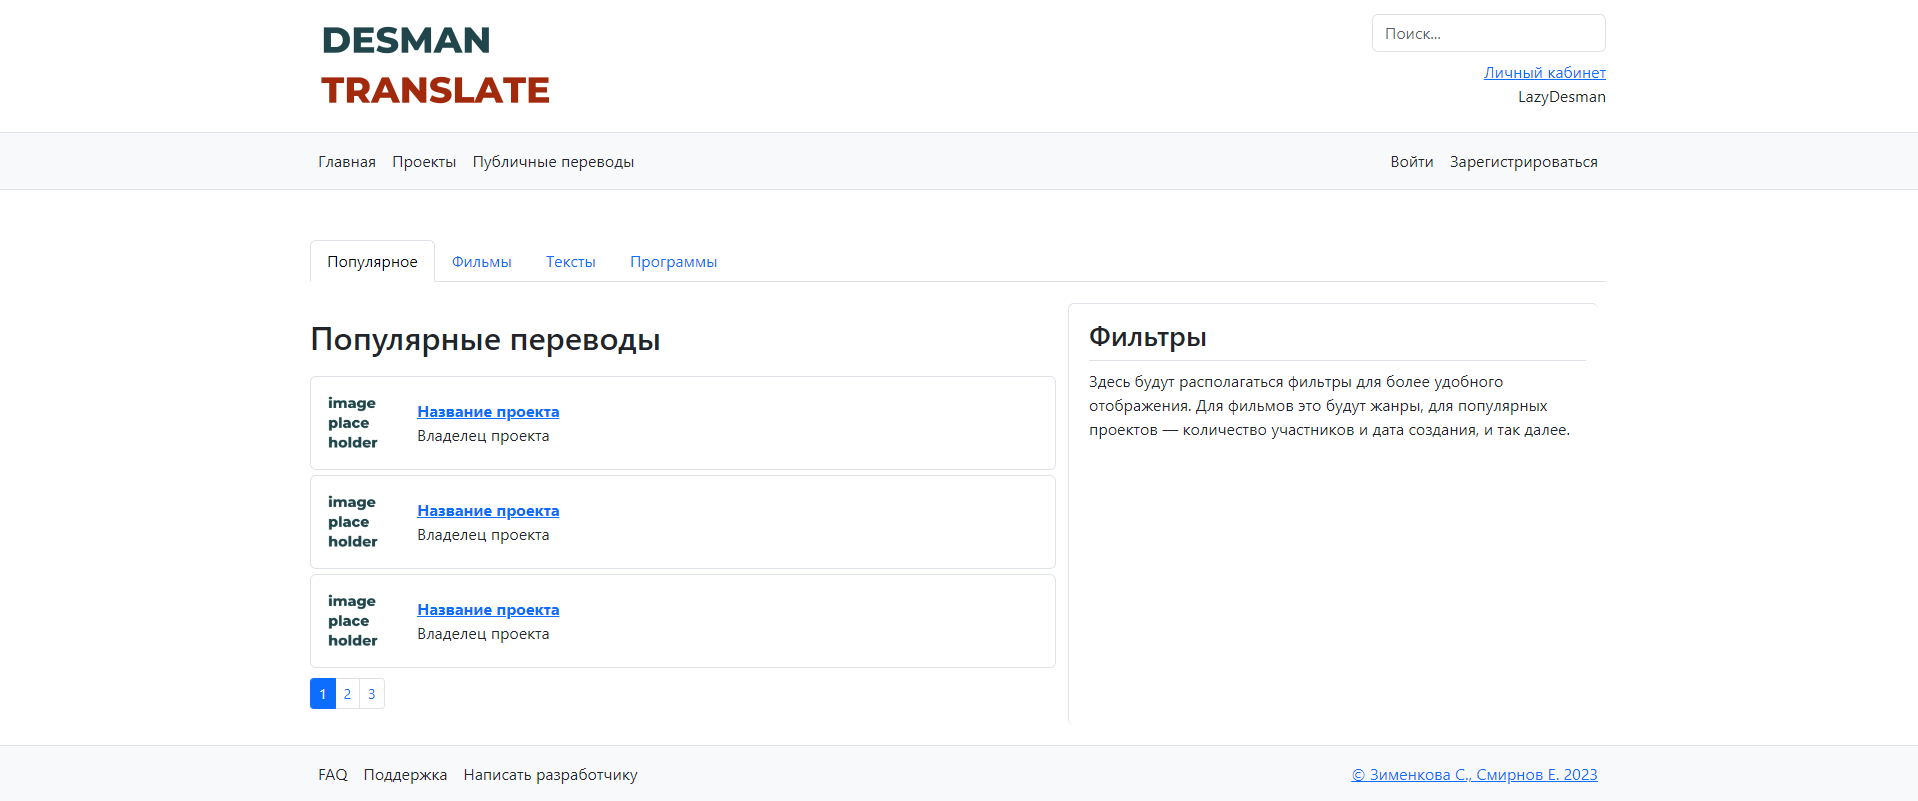
\includegraphics[width=400px]{public1.png}
\caption{Страница популярных переводов.}
\label{fig:public1}
\end{figure}

\begin{figure}[h]
\centering
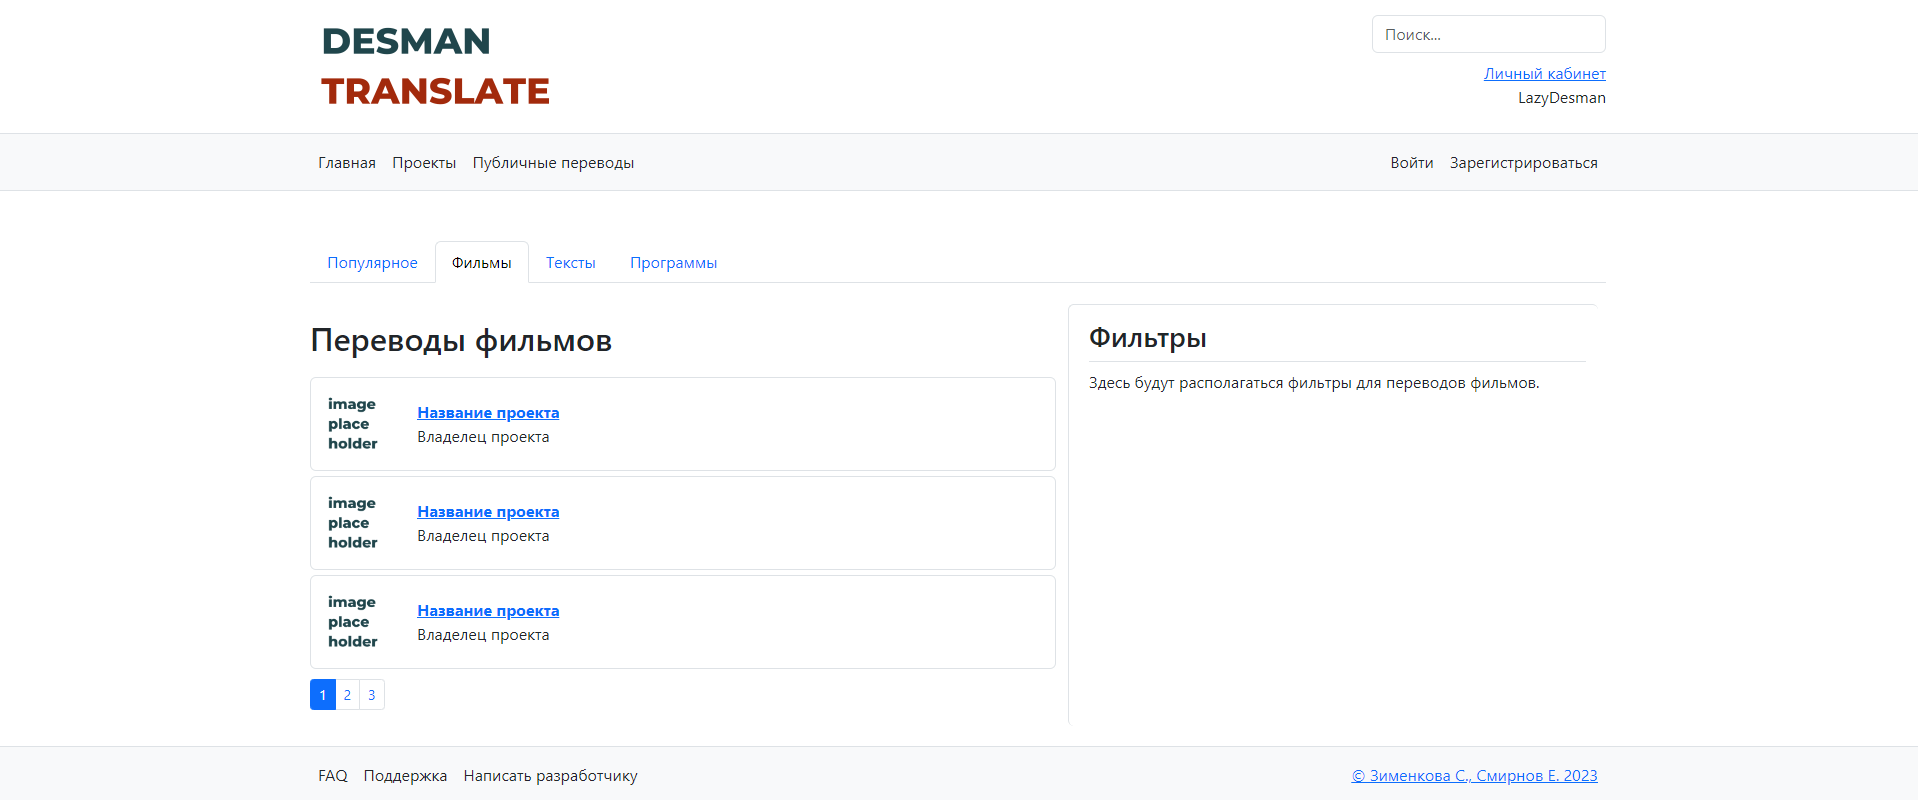
\includegraphics[width=400px]{public2.png}
\caption{Преводы фильмов.}
\label{fig:public2}
\end{figure}


\begin{figure}[h]
\centering
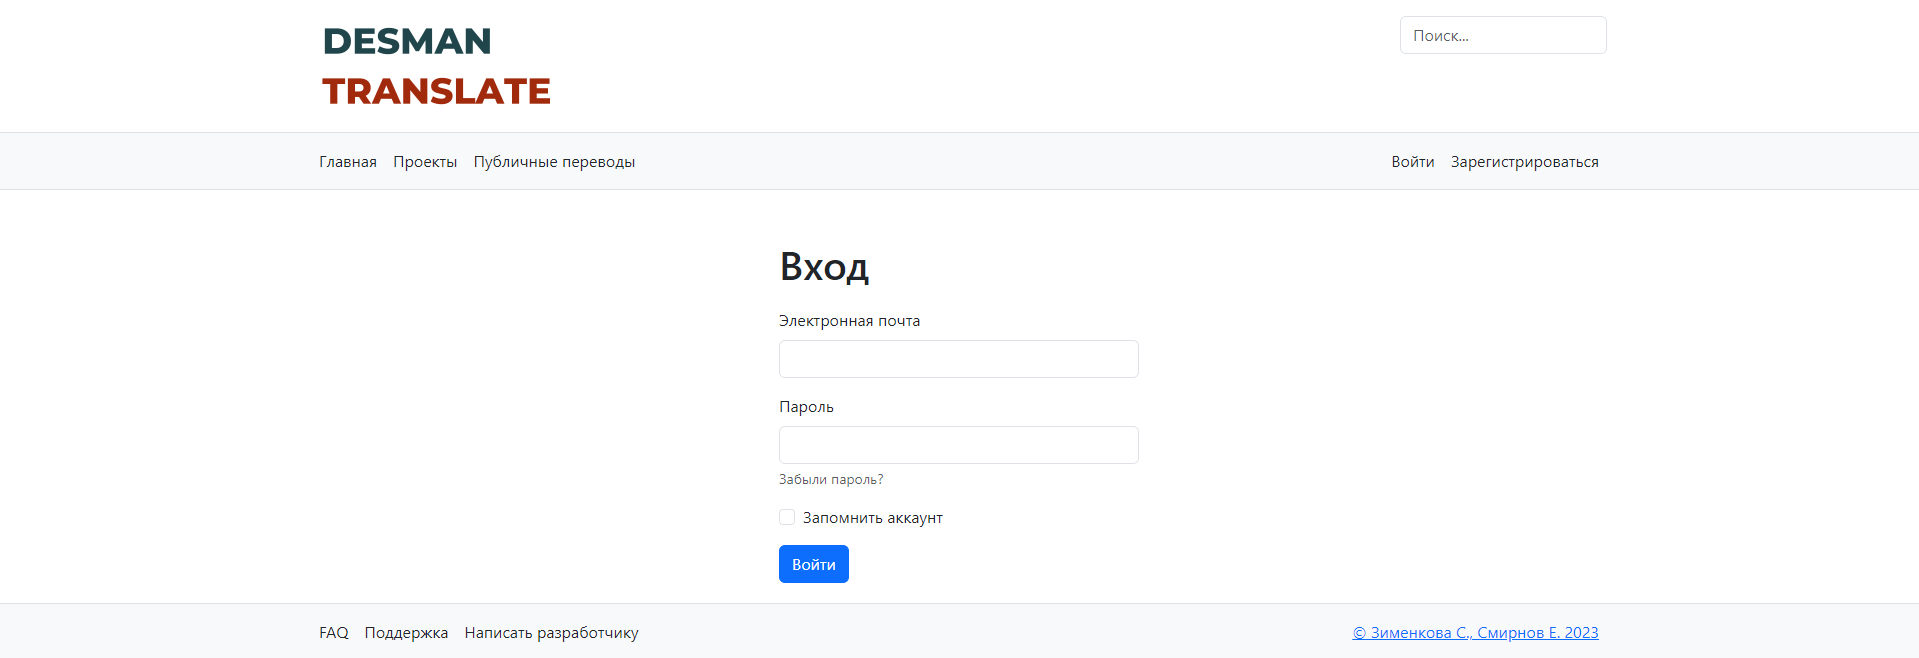
\includegraphics[width=400px]{login.png}
\caption{Вход в аккаунт.}
\label{fig:login}
\end{figure}

\begin{figure}[h]
\centering
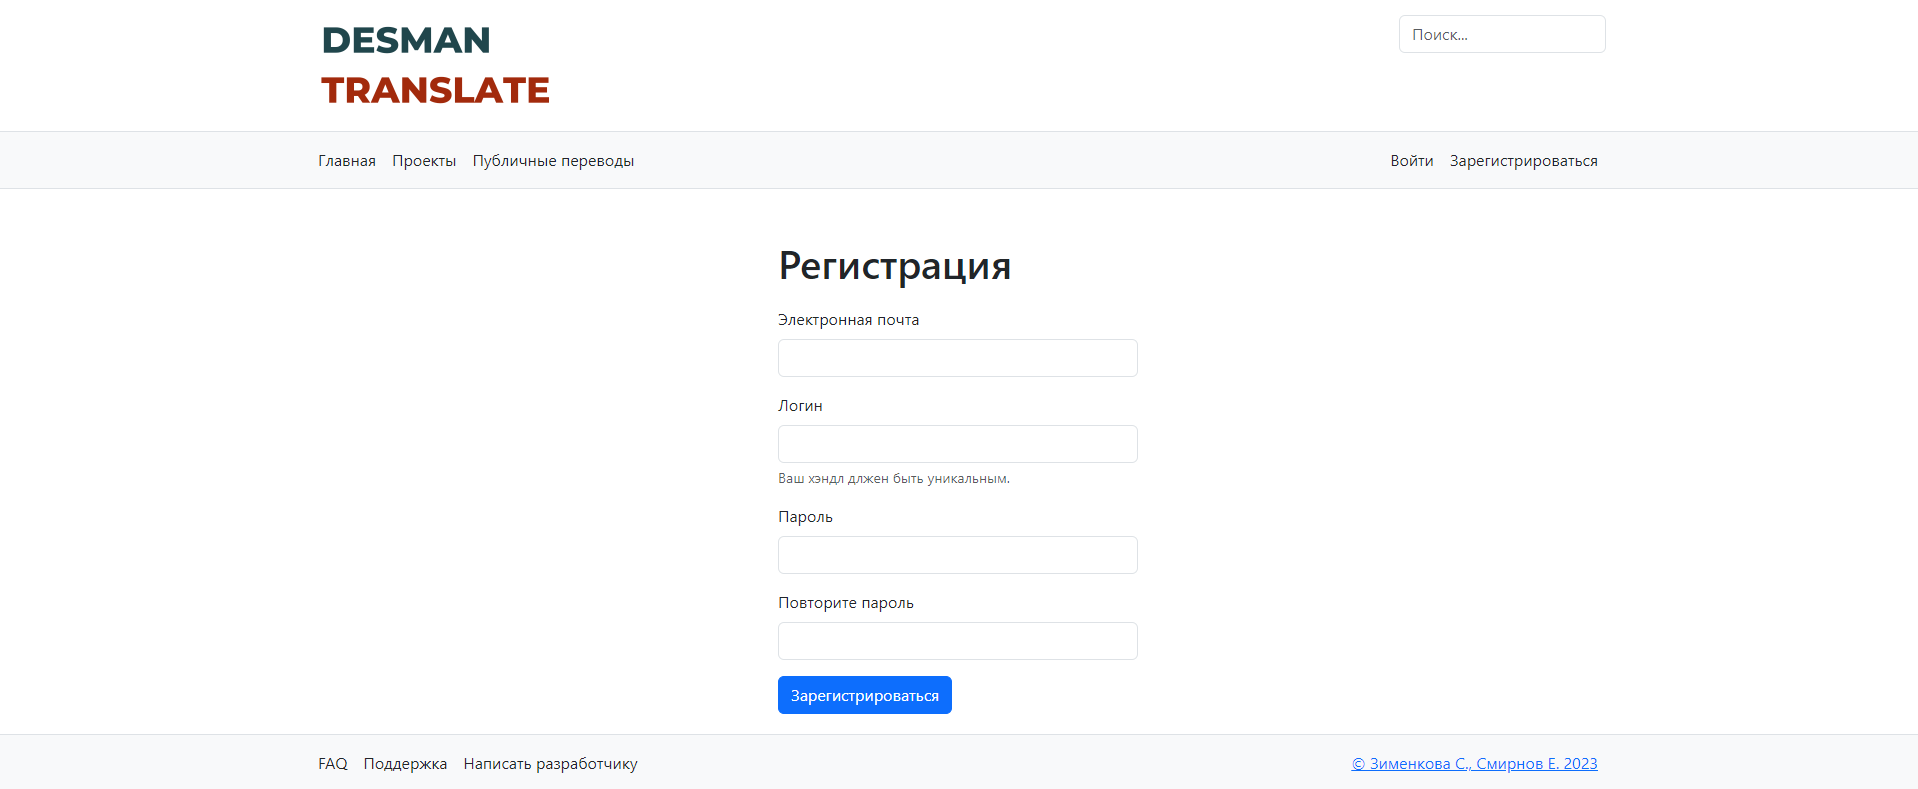
\includegraphics[width=400px]{signup.png}
\caption{Регистрация.}
\label{fig:signup}
\end{figure}


\begin{figure}[h]
\centering
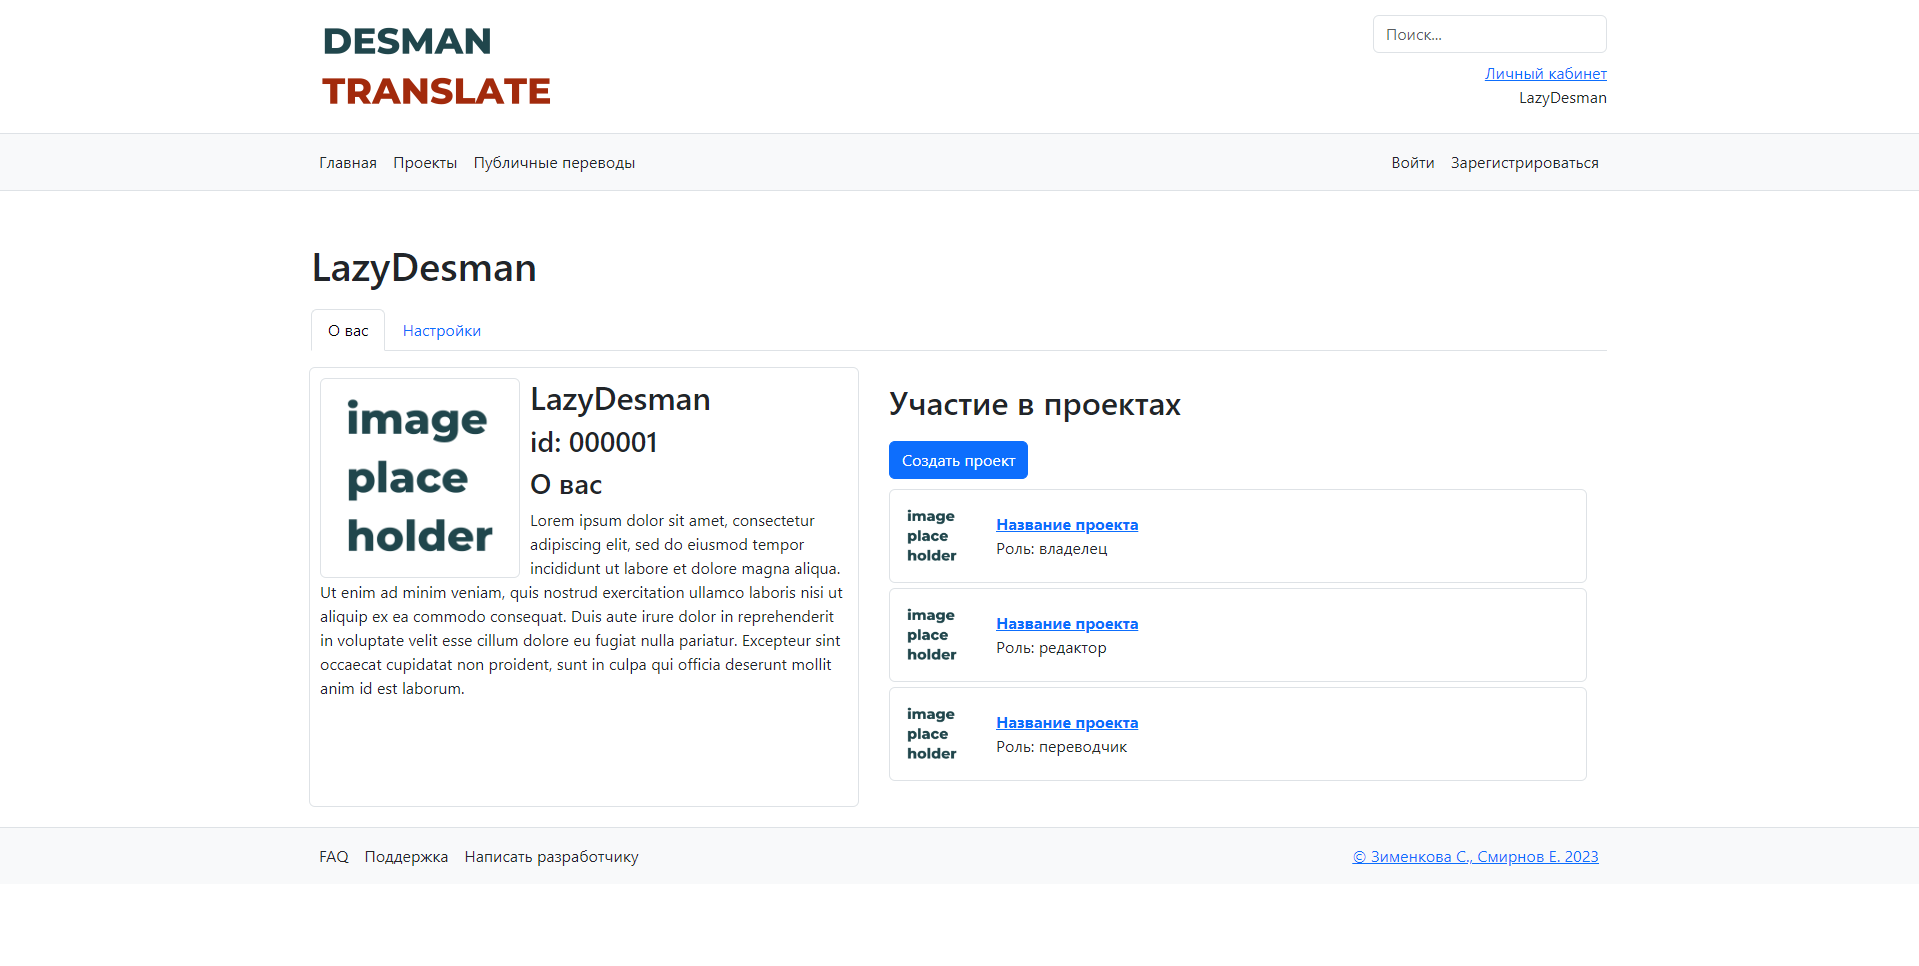
\includegraphics[width=400px]{user.png}
\caption{Личный кабинет пользователя.}
\label{fig:user}
\end{figure}

\begin{figure}[h]
\centering
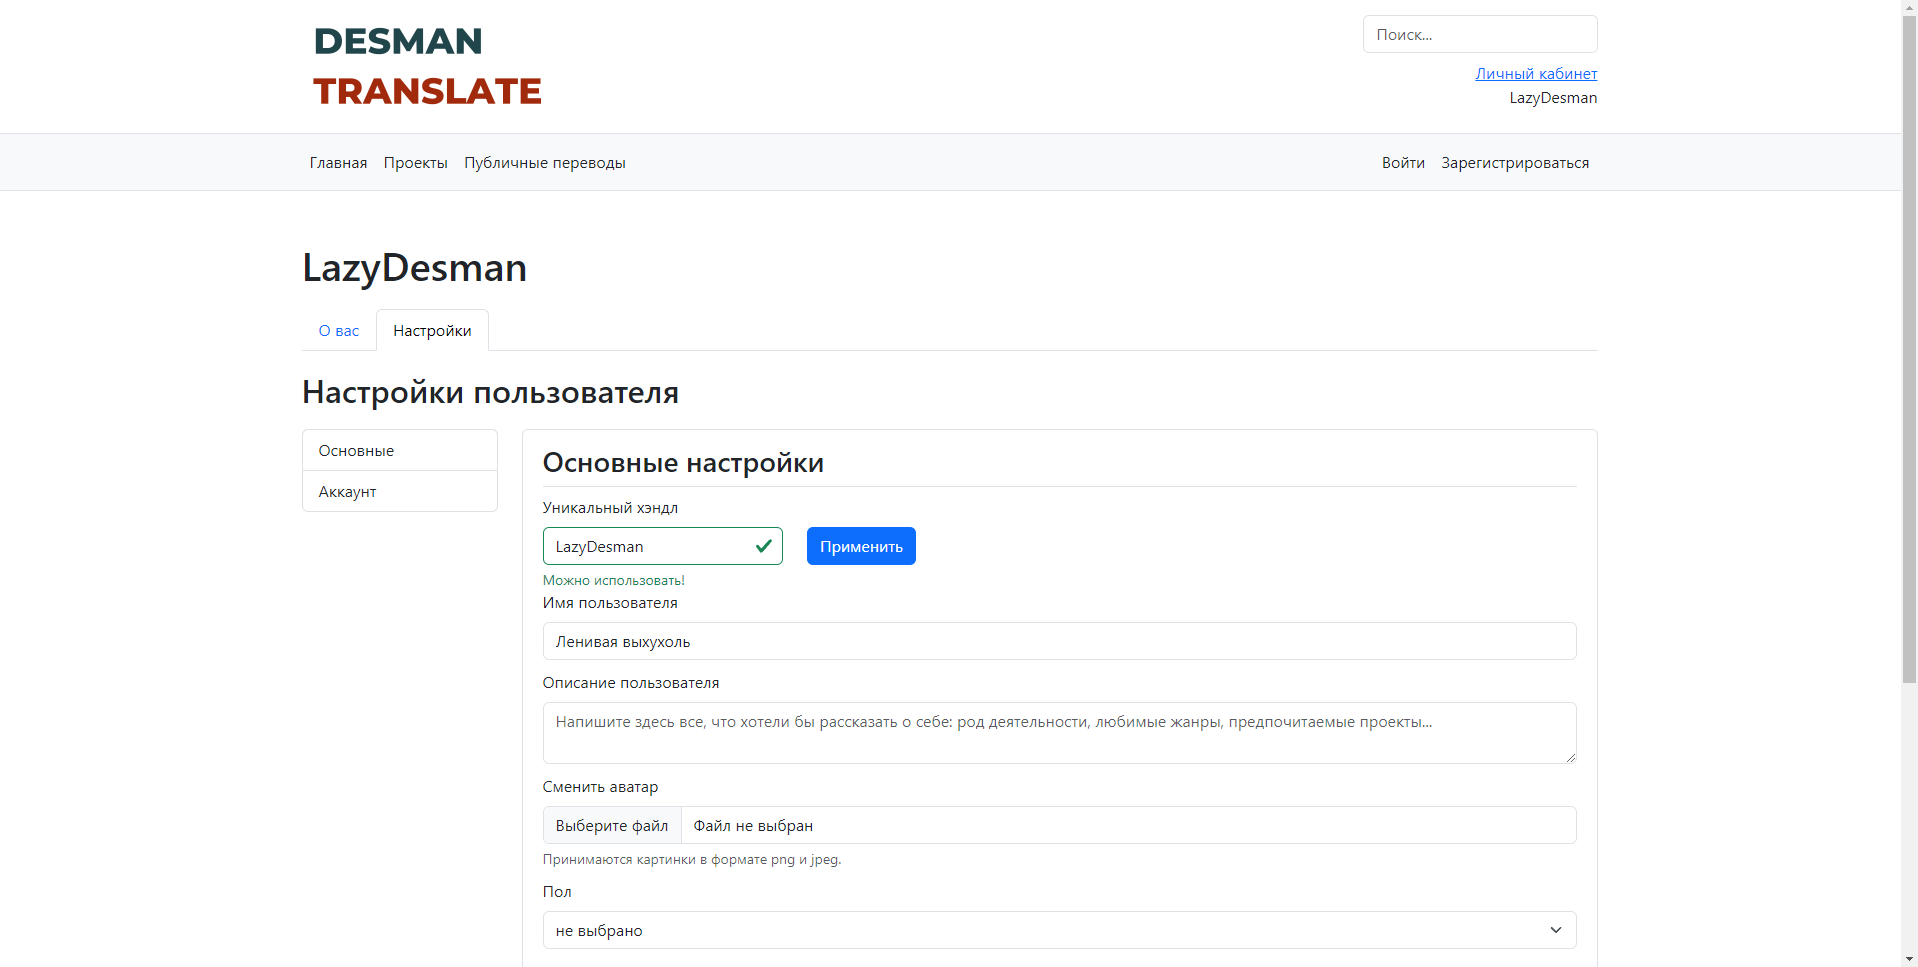
\includegraphics[width=400px]{usersettings1.png}

\includegraphics[width=400px]{usersettings2.png}
\caption{Настройки в личном кабинете пользователя.}
\label{fig:usersettings}
\end{figure}


\begin{figure}[h]
\centering
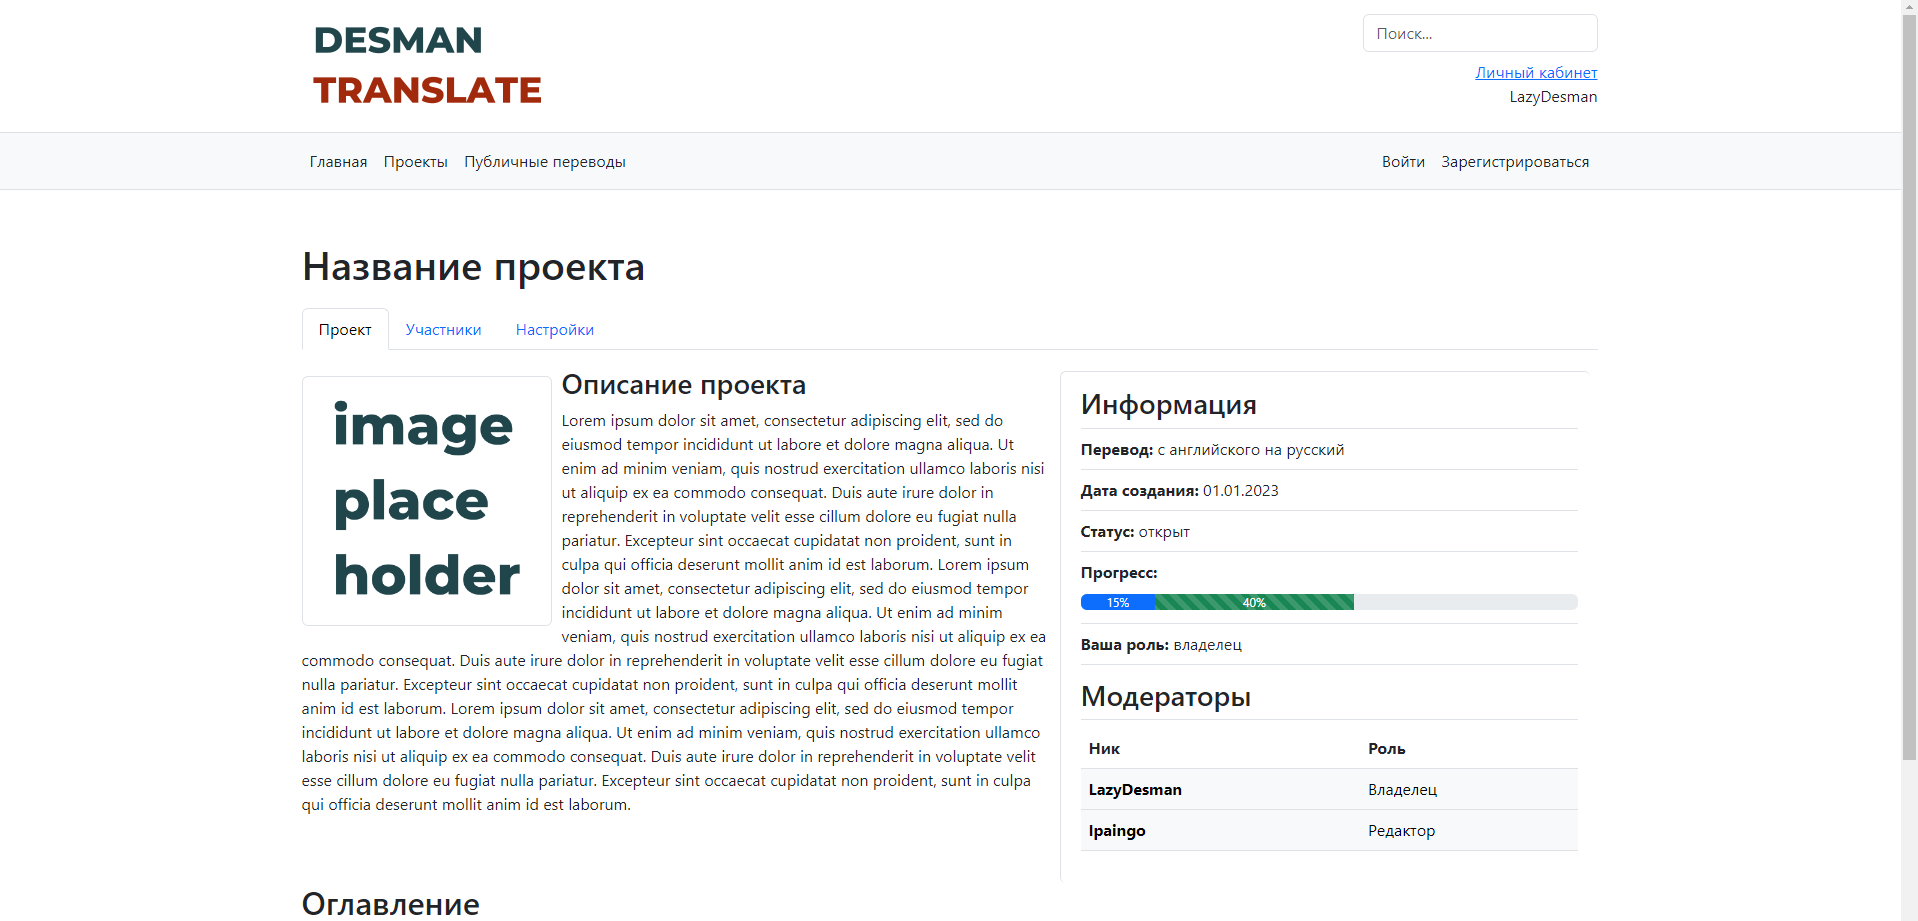
\includegraphics[width=400px]{projectpage1.png}

\includegraphics[width=400px]{projectpage2.png}
\caption{Страница проекта.}
\label{fig:projectpage}
\end{figure}

\begin{figure}[h]
\centering
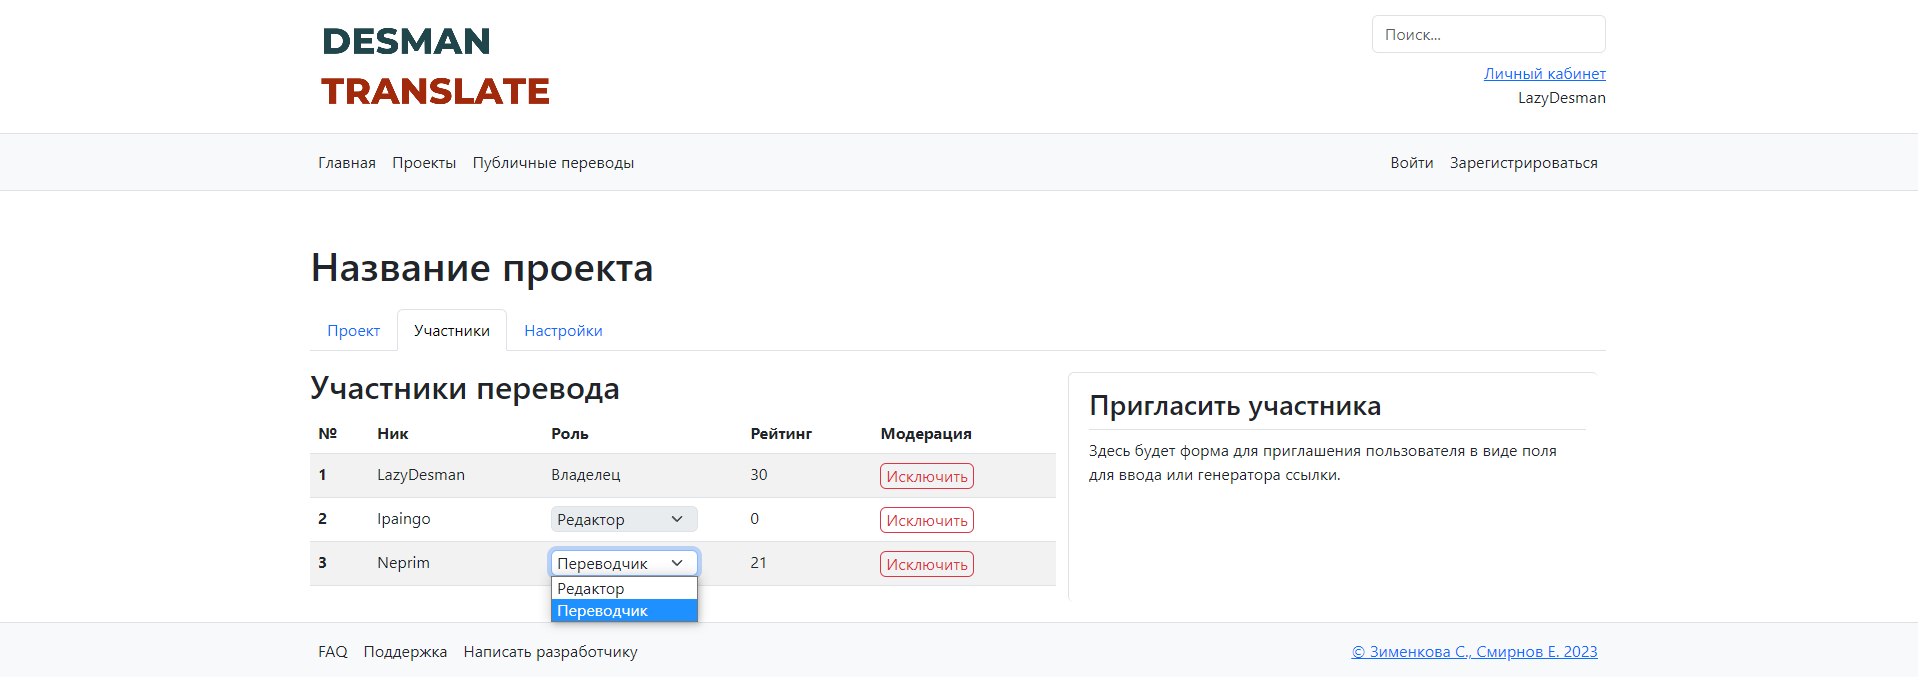
\includegraphics[width=400px]{members.png}
\caption{Участники проекта.}
\label{fig:members}
\end{figure}

\begin{figure}[h]
\centering
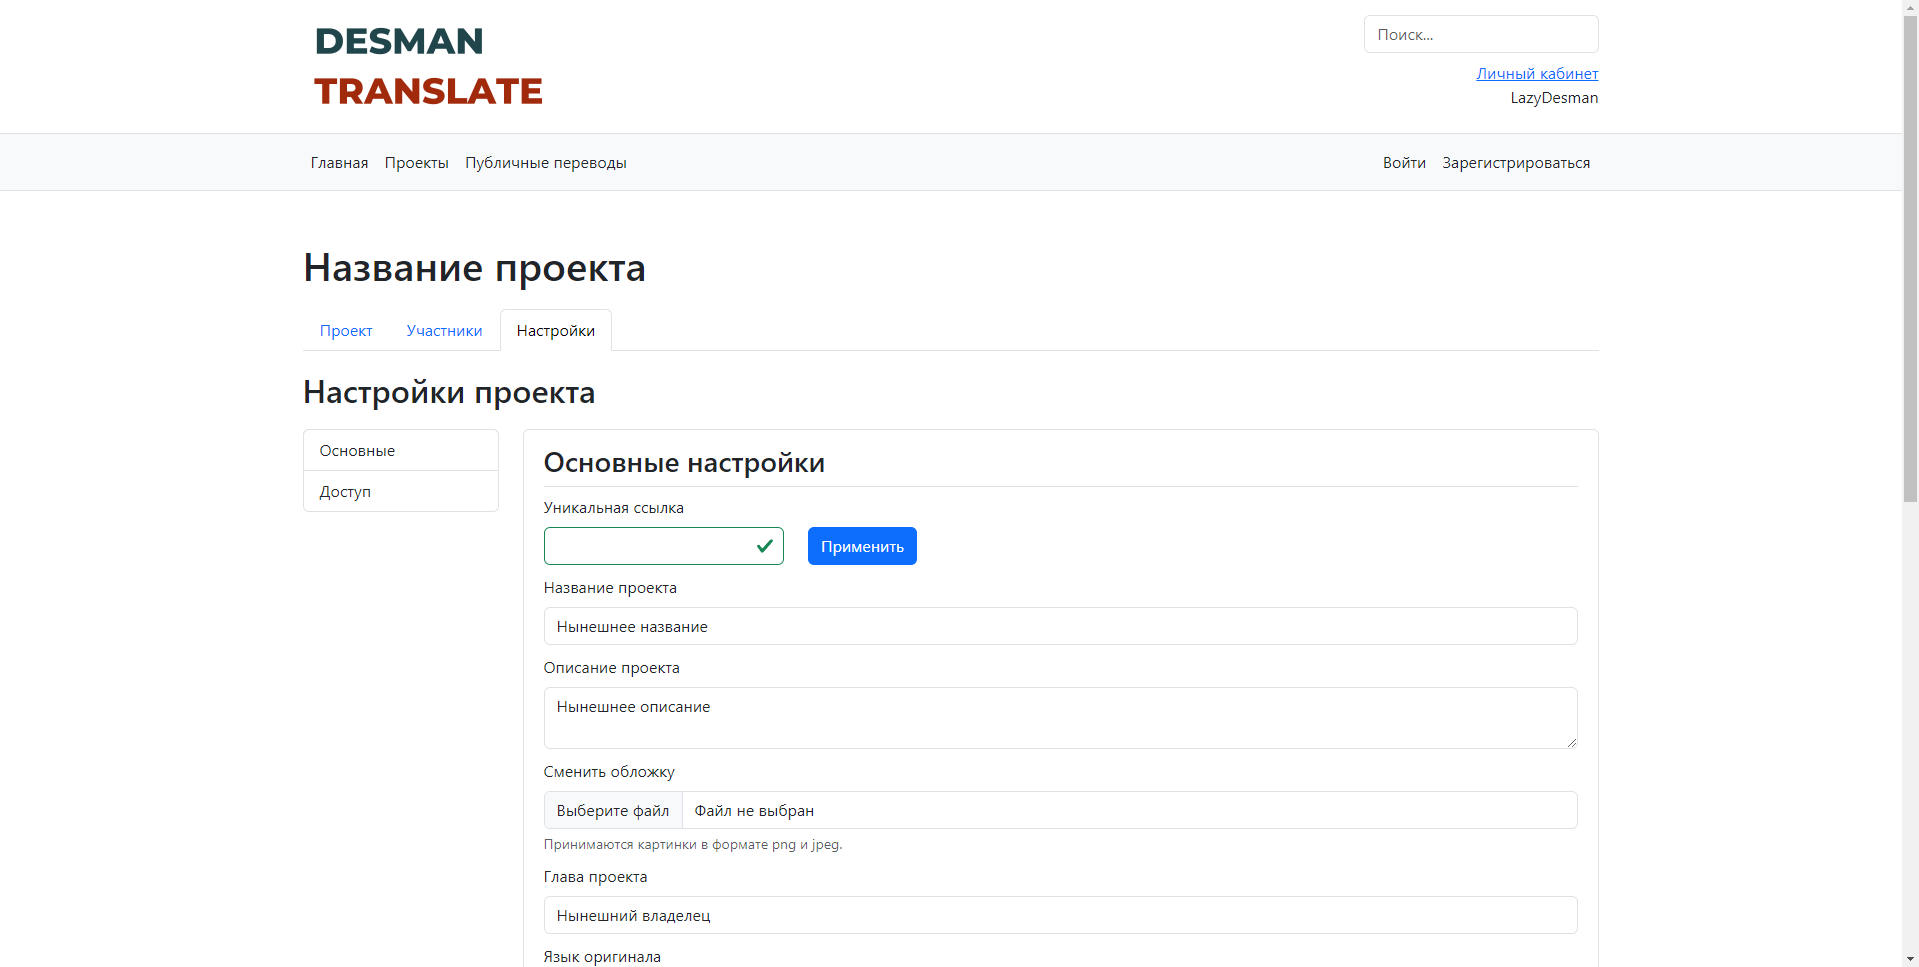
\includegraphics[width=400px]{settings1.png}
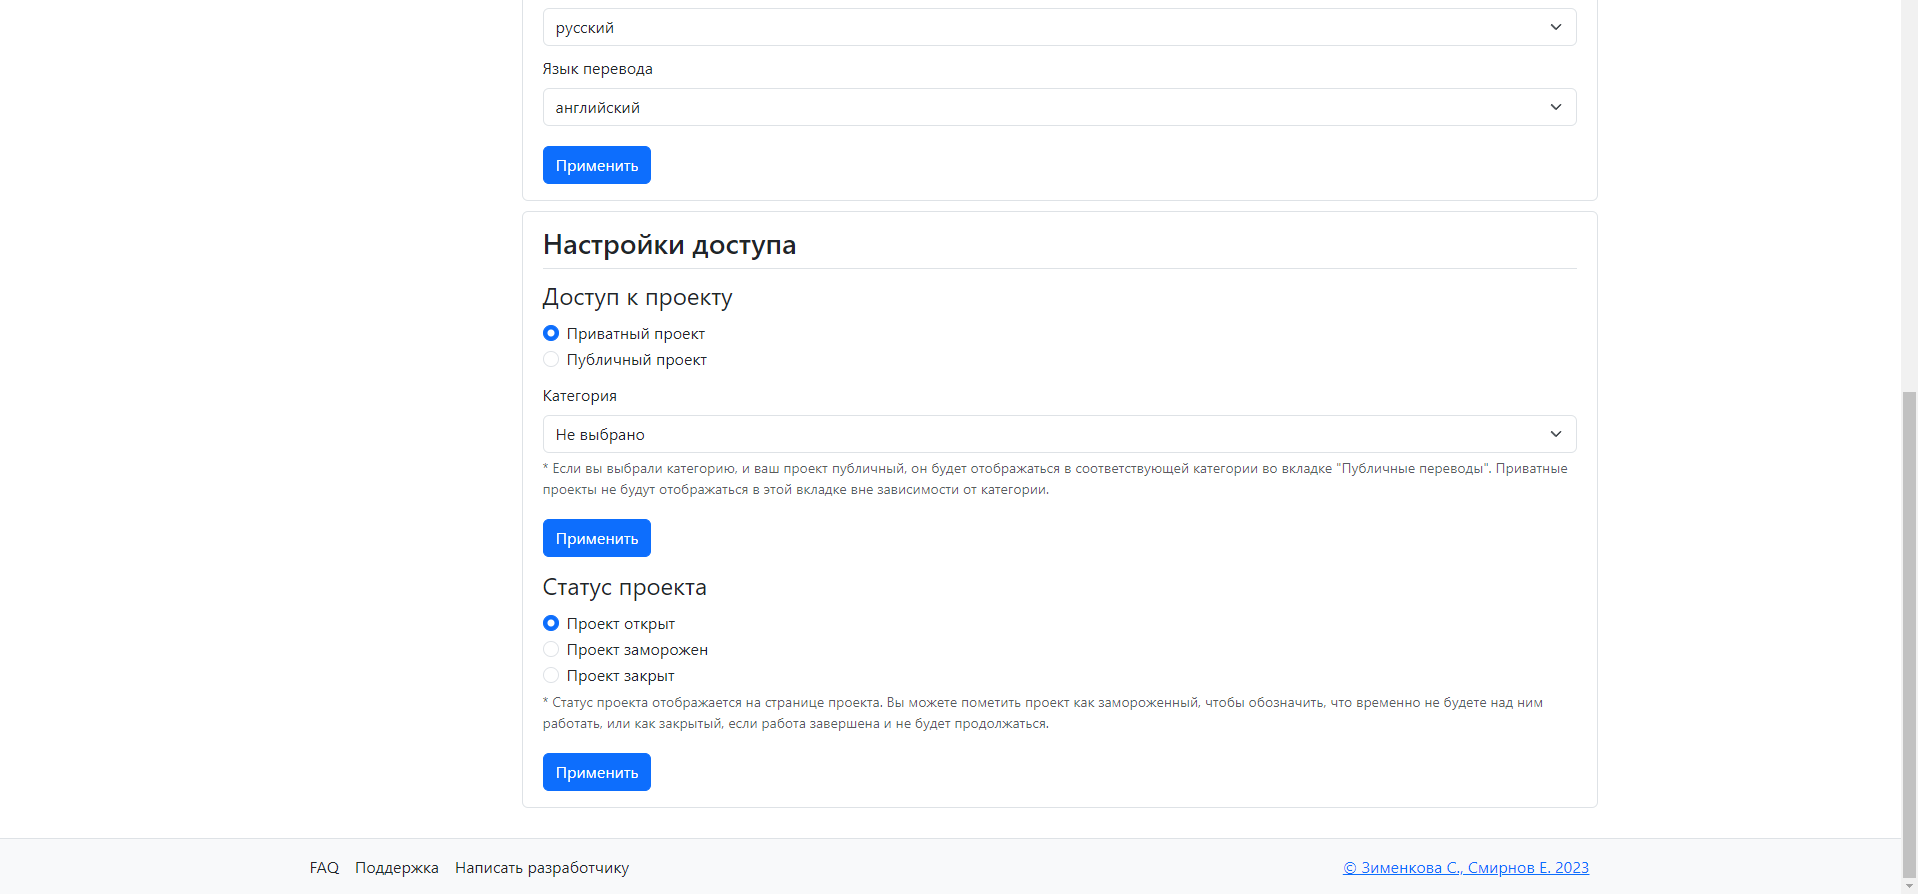
\includegraphics[width=400px]{settings2.png}
\caption{Настройки проекта.}
\label{fig:settings}
\end{figure}

\begin{figure}[h]
\centering
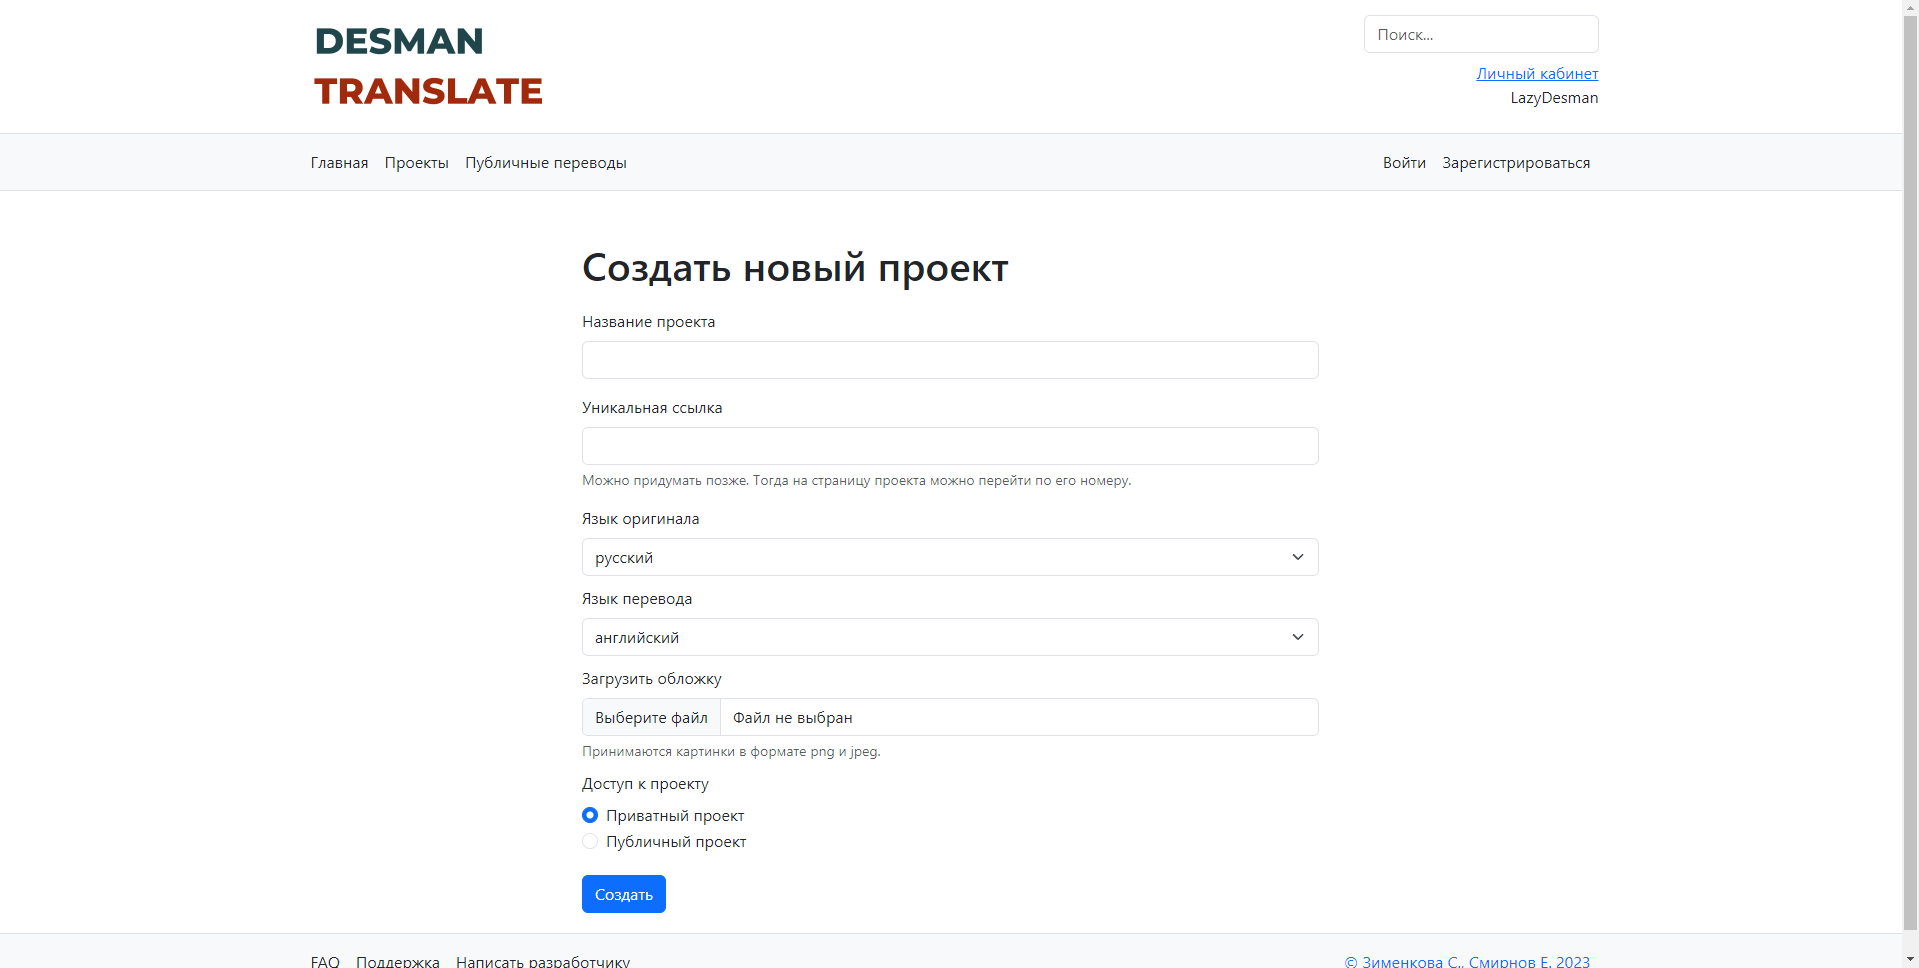
\includegraphics[width=400px]{newproject.png}
\caption{Форма для создания нового проекта.}
\label{fig:newproject}
\end{figure}


\begin{figure}[h]
\centering
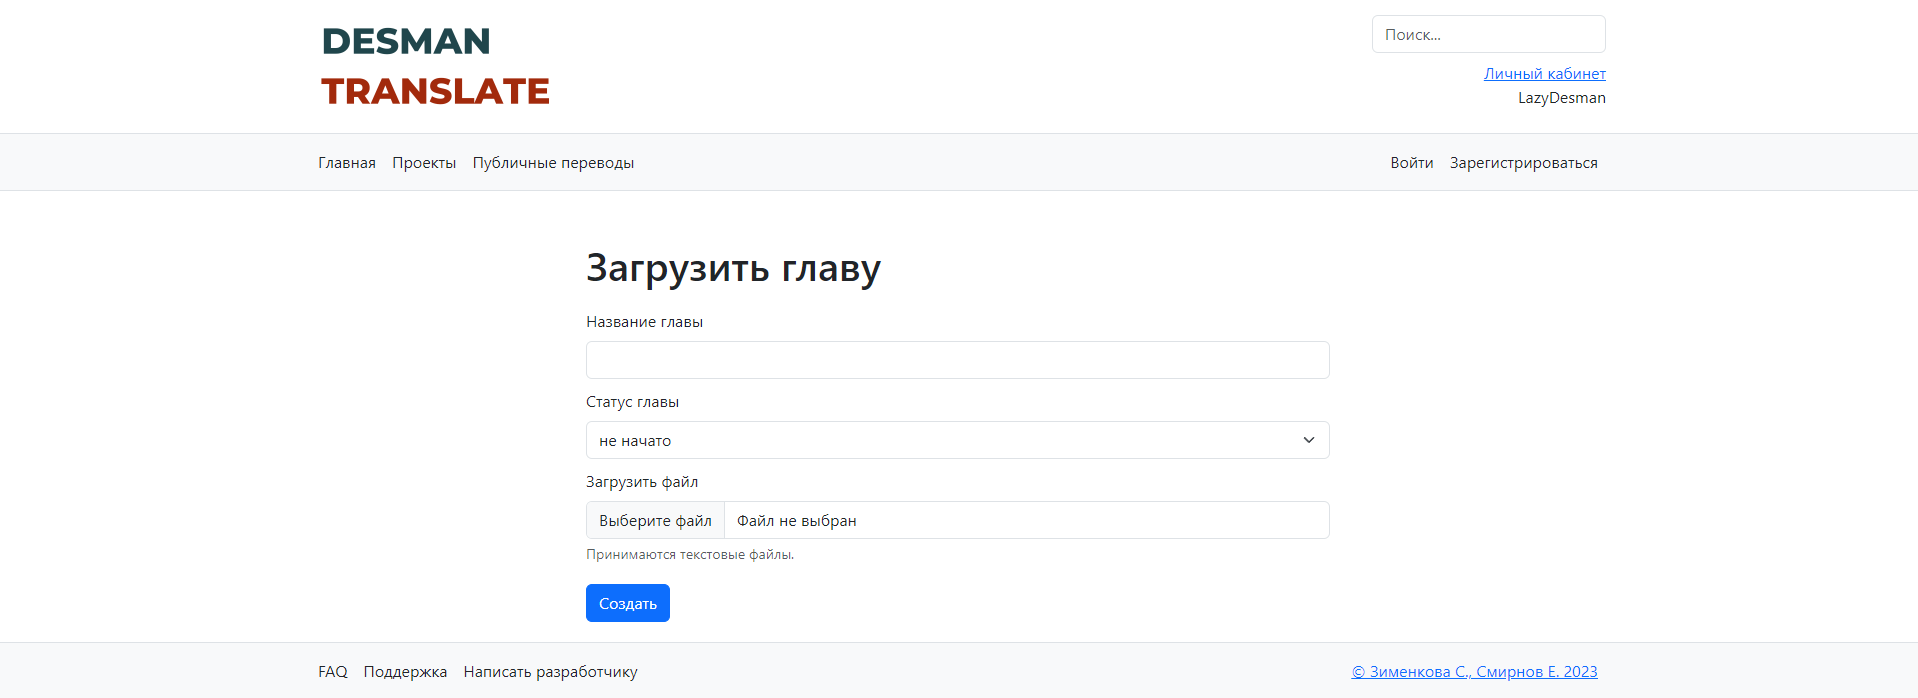
\includegraphics[width=400px]{addchapter.png}
\caption{Страница для загрузки новых глав.}
\label{fig:addchapter}
\end{figure}

%%% Приложение        %%%
%%%                   %%%
%%%%%%%%%%%%%%%%%%%%%%%%%
 

\end{document}